\documentclass[preprint,review,12pt,authoryear]{static/elsarticle}

% Use the document width more effectively.
\usepackage[margin=2.5cm]{geometry}

% Enable captions for figures and tables.
\usepackage{caption}

% Enable diagonal lines in tables.
\usepackage{static/slashbox}

% Enable multiple lines in a table row
\usepackage{multirow}

% Make opening quotes look different than closing quotes.
\usepackage[english=american]{csquotes}
\MakeOuterQuote{"}

% Define helper commands.
\usepackage{bm}
\newcommand{\mat}[1]{\bm{#1}}
\newcommand{\norm}[1]{\left\lVert#1\right\rVert}
\newcommand{\thead}[1]{\textbf{#1}}

\begin{document}

\begin{frontmatter}

\journal{Transportation Research Part E}
\title{Real-time Demand Forecasting for an Urban Delivery Platform}

\author[WHU]{Alexander Hess\fnref{emails}\fnref{corresponding}}
\author[WHU]{Stefan Spinler\fnref{emails}}
\author[MIT]{Matthias Winkenbach\fnref{emails}}
\address[WHU]{
WHU - Otto Beisheim School of Management,
Burgplatz 2, 56179 Vallendar, Germany
}
\address[MIT]{
Massachusetts Institute of Technology,
77 Massachusetts Avenue, Cambridge, MA 02139, United States
}
\fntext[email]{
Emails:
    alexander.hess@whu.edu,
    stefan.spinler@whu.edu,
    mwinkenb@mit.edu
}

\fntext[corresponding]{
The corresponding author is Alexander Hess.
Use the provided email.
}

\begin{abstract}
Meal delivery platforms like Uber Eats shape the landscape in cities around the world.
This paper addresses forecasting demand on a grid into the short-term future,
    enabling, for example, predictive routing applications.
We propose an approach incorporating
    both classical forecasting and machine learning methods
    and adapt model evaluation and selection to typical demand:
        intermittent with a double-seasonal pattern.
An empirical study shows that
    an exponential smoothing based method trained on past demand data alone
        achieves optimal accuracy,
    if at least two months are on record.
With a more limited demand history,
    machine learning is shown
    to yield more accurate prediction results than classical methods.
\end{abstract}

\begin{keyword}
demand forecasting \sep
intermittent demand \sep
machine learning \sep
urban delivery platform
\end{keyword}

\end{frontmatter}
\newpage

\section{Introduction}
\label{intro}
\section{Literature Review}
\label{lit}
\subsection{Demand Forecasting with Classical Forecasting Methods}
\label{class_methods}

Forecasting became a formal discipline starting in the 1950s and has its
    origins in the broader field of statistics.
\cite{hyndman2018} provide a thorough overview of the concepts and methods
    established, and \cite{ord2017} indicate business-related applications
    such as demand forecasting.
These "classical" forecasting methods share the characteristic that they are
    trained over the entire $Y$ first.
Then, for prediction, the forecaster specifies the number of time steps for
    which he wants to generate forecasts.
That is different for ML models.

\subsubsection{Na\"{i}ve Methods, Moving Averages, and Exponential Smoothing.}
\label{ets}

Simple forecasting methods are often employed as a benchmark for more
    sophisticated ones.
The so-called na\"{i}ve and seasonal na\"{i}ve methods forecast the next time
    step in a time series, $y_{T+1}$, with the last observation, $y_T$,
    and, if a seasonal pattern is present, with the observation $k$ steps
    before, $y_{T+1-k}$.
As variants, both methods can be generalized to include drift terms in the
    presence of a trend or changing seasonal amplitude.

If a time series exhibits no trend, a simple moving average (SMA) is a
    generalization of the na\"{i}ve method that is more robust to outliers.
It is defined as follows: $\hat{y}_{T+1} = \frac{1}{h} \sum_{i=T-h}^{T} y_i$
    where $h$ is the horizon over which the average is calculated.
If a time series exhibits a seasonal pattern, setting $h$ to a multiple of the
    periodicity $k$ suffices that the forecast is unbiased.

Starting in the 1950s, another popular family of forecasting methods,
    so-called exponential smoothing methods, was introduced by
    \cite{brown1959}, \cite{holt1957}, and \cite{winters1960}.
The idea is that forecasts $\hat{y}_{T+1}$ are a weighted average of past
    observations where the weights decay over time; in the case of the simple
    exponential smoothing (SES) method we obtain:
$
\hat{y}_{T+1} = \alpha y_T + \alpha (1 - \alpha) y_{T-1}
                + \alpha (1 - \alpha)^2 y_{T-2}
                + \dots + \alpha (1 - \alpha)^{T-1} y_{1}
$
where $\alpha$ (with $0 \le \alpha \le 1$) is a smoothing parameter.

Exponential smoothing methods are often expressed in an alternative component
    form that consists of a forecast equation and one or more smoothing
    equations for unobservable components.
Below, we present a generalization of SES, the so-called Holt-Winters'
    seasonal method, in an additive formulation.
$\ell_t$, $b_t$, and $s_t$ represent the unobservable level, trend, and
    seasonal components inherent in $y_t$, and $\beta$ and $\gamma$ complement
    $\alpha$ as smoothing parameters:
\begin{align*}
\hat{y}_{t+1} & = \ell_t + b_t + s_{t+1-k} \\
\ell_t        & = \alpha(y_t - s_{t-k}) + (1 - \alpha)(\ell_{t-1} + b_{t-1}) \\
b_t           & = \beta (\ell_{t} - \ell_{t-1}) + (1 - \beta) b_{t-1} \\
s_t           & = \gamma (y_t - \ell_{t-1} - b_{t-1}) + (1-\gamma)s_{t-k}
\end{align*}
With $b_t$, $s_t$, $\beta$, and $\gamma$ removed, this formulation reduces to
    SES.
Distinct variations exist: Besides the three components, \cite{gardner1985}
    add dampening for the trend, \cite{pegels1969} provides multiplicative
    formulations, and \cite{taylor2003} adds dampening to the latter.
The accuracy measure commonly employed is the sum of squared errors between
    the observations and their forecasts.

Originally introduced by \cite{assimakopoulos2000}, \cite{hyndman2003} show
    how the Theta method can be regarded as an equivalent to SES with a drift
    term.
We mention this method here only because \cite{bell2018} emphasize that it
    performs well at Uber.
However, in our empirical study, we find that this is not true in general.

\cite{hyndman2002} introduce statistical processes, so-called innovations	
    state-space models, to generalize the methods in this sub-section.
They call this family of models ETS as they capture error, trend, and seasonal
    terms.
Linear and additive ETS models have a structure like so:
\begin{align*}
y_t       & = \vec{w} \cdot \vec{x}_{t-1} + \epsilon_t \\
\vec{x_t} & = \mat{F} \vec{x}_{t-1} + \vec{g} \epsilon_t
\end{align*}
$y_t$ denote the observations as before while $\vec{x}_t$ is a state vector of
    unobserved components.
$\epsilon_t$ is a white noise series and the matrix $\mat{F}$ and the vectors
    $\vec{g}$ and $\vec{w}$ contain a model's coefficients.
Just as the models in the next sub-section, ETS models are commonly fitted
    with maximum likelihood and evaluated using information theoretical
    criteria against historical data.
We refer to \cite{hyndman2008b} for a thorough summary.

\subsubsection{Autoregressive Integrated Moving Averages}
\label{arima}

\cite{box1962}, \cite{box1968}, and more papers by the same authors in the
    1960s introduce a type of model where observations correlate with their
    neighbors and refer to them as autoregressive integrated moving average
    (ARIMA) models for stationary time series.
For a thorough overview, we refer to \cite{box2015} and \cite{brockwell2016}.

A time series $y_t$ is stationary if its moments are independent of the
    point in time where it is observed.
A typical example is a white noise $\epsilon_t$ series.
Therefore, a trend or seasonality implies non-stationarity.
\cite{kwiatkowski1992} provide a test to check the null hypothesis of
    stationary data.
To obtain a stationary time series, one chooses from several techniques:
First, to stabilize a changing variance (i.e., heteroscedasticity), one
    applies a Box-Cox transformation (e.g., $log$) as first suggested by
    \cite{box1964}.
Second, to factor out a trend (or seasonal) pattern, one computes differences
    of consecutive (or of lag $k$) observations or even differences thereof.
Third, it is also common to pre-process $y_t$ with one of the decomposition
    methods mentioned in Sub-section \ref{stl} below with an ARIMA model
    then trained on an adjusted $y_t$.

In the autoregressive part, observations are modeled as linear combinations of
    its predecessors.
Formally, an $AR(p)$ model is defined with a drift term $c$, coefficients
    $\phi_i$ to be estimated (where $i$ is an index with $0 < i \leq p$), and
    white noise $\epsilon_t$ like so:
$
AR(p): \ \
y_t = c + \phi_1 y_{t-1} + \phi_2 y_{t-2} + \dots + \phi_p y_{t-p}
      + \epsilon_t
$.
The moving average part considers observations to be regressing towards a
    linear combination of past forecasting errors.
Formally, a $MA(q)$ model is defined with a drift term $c$, coefficients
    $\theta_j$ to be estimated, and white noise terms $\epsilon_t$ (where $j$
    is an index with $0 < j \leq q$) as follows:
$
MA(q): \ \
y_t = c + \epsilon_t + \theta_1 \epsilon_{t-1} + \theta_2 \epsilon_{t-2}
      + \dots + \theta_q \epsilon_{t-q}
$.
Finally, an $ARIMA(p,d,q)$ model unifies both parts and adds differencing
    where $d$ is the degree of differences and the $'$ indicates differenced
    values:
$
ARIMA(p,d,q): \ \
y'_t = c + \phi_1 y'_{t-1} + \dots + \phi_p y'_{t-p} + \theta_1 \epsilon_{t-1}
       + \dots + \theta_q \epsilon_{t-q} + \epsilon_{t}
$.

$ARIMA(p,d,q)$ models are commonly fitted with maximum likelihood estimation.
To find an optimal combination of the parameters $p$, $d$, and $q$, the
    literature suggests calculating an information theoretical criterion
    (e.g., Akaike's Information Criterion) that evaluates the fit on
    historical data.
\cite{hyndman2008a} provide a step-wise heuristic to choose $p$, $d$, and $q$,
    that also decides if a Box-Cox transformation is to be applied, and if so,
    which one.
To obtain a one-step-ahead forecast, the above equation is reordered such
    that $t$ is substituted with $T+1$.
For forecasts further into the future, the actual observations are
    subsequently replaced by their forecasts.    
Seasonal ARIMA variants exist; however, the high frequency $k$ in the kind of
    demand a UDP faces typically renders them impractical as too many
    coefficients must be estimated.

\subsubsection{Seasonal and Trend Decomposition using Loess}
\label{stl}

A time series $y_t$ may exhibit different types of patterns; to fully capture
    each of them, the series must be decomposed.
Then, each component is forecast with a distinct model.
Most commonly, the components are the trend $t_t$, seasonality $s_t$, and
    remainder $r_t$.
They are themselves time series, where only $s_t$ exhibits a periodicity $k$.
A decomposition may be additive (i.e., $y_t = s_t + t_t + r_t$) or
    multiplicative (i.e., $y_t = s_t * t_t * r_t$); the former assumes that
    the effect of the seasonal component is independent of the overall level
    of $y_t$ and vice versa.
The seasonal component is centered around $0$ in both cases such that its
    removal does not affect the level of $y_t$.
Often, it is sufficient to only seasonally adjust the time series, and model
    the trend and remainder together, for example, as $a_t = y_t - s_t$ in the
    additive case.

Early approaches employed moving averages (cf., Sub-section \ref{ets}) to
    calculate a trend component, and, after removing that from $y_t$, averaged
    all observations of the same seasonal lag to obtain the seasonal
    component.
The downsides of this are the subjectivity in choosing the window lengths for
    the moving average and the seasonal averaging, the incapability of the
    seasonal component to vary its amplitude over time, and the missing
    handling of outliers.

The X11 method developed at the U.S. Census Bureau and described in detail by
    \cite{dagum2016} overcomes these disadvantages.
However, due to its background in economics, it is designed primarily for
    quarterly or monthly data, and the change in amplitude over time cannot be
    controlled.
Variants of this method are the SEATS decomposition by the Bank of Spain and
    the newer X13-SEATS-ARIMA method by the U.S. Census Bureau.
Their main advantages stem from the fact that the models calibrate themselves
    according to statistical criteria without manual work for a statistician
    and that the fitting process is robust to outliers.

\cite{cleveland1990} introduce a seasonal and trend decomposition using a
    repeated locally weighted regression - the so-called Loess procedure - to
    smoothen the trend and seasonal components, which can be viewed as a
    generalization of the methods above and is denoted by the acronym
    \gls{stl}.
In contrast to the X11, X13, and SEATS methods, the STL supports seasonalities
    of any lag $k$ that must, however, be determined with additional
    statistical tests or set with out-of-band knowledge by the forecaster
    (e.g., hourly demand data implies $k = 24 * 7 = 168$ assuming customer
    behavior differs on each day of the week).
Moreover, the seasonal component's rate of change, represented by the $ns$
    parameter and explained in detail with Figure \ref{f:stl} in Section
    \ref{decomp}, must be set by the forecaster as well, while the trend's
    smoothness may be controlled via setting a non-default window size.
Outliers are handled by assignment to the remainder such that they do not
    affect the trend and seasonal components.
In particular, the manual input needed to calibrate the STL explains why only
    the X11, X13, and SEATS methods are widely used by practitioners.
However, the widespread adoption of concepts like cross-validation (cf.,
    Sub-section \ref{cv}) in recent years enables the usage of an automated
    grid search to optimize the parameters.
The STL's usage within a grid search is facilitated even further by its being
    computationally cheaper than the other methods discussed.

\subsection{Demand Forecasting with Machine Learning Methods}
\label{ml_methods}

ML methods have been employed in all kinds of prediction tasks in recent
    years.
In this section, we restrict ourselves to the models that performed well in
    our study: Random Forest (\gls{rf}) and Support Vector Regression
    (\gls{svr}).
RFs are in general well-suited for datasets without a priori knowledge about
    the patterns, while SVR is known to perform well on time series data, as
    shown by \cite{hansen2006} in general and \cite{bao2004} specifically for
    intermittent demand.
Gradient Boosting, another popular ML method, was consistently outperformed by
    RFs, and artificial neural networks require an amount of data
    exceeding what our industry partner has by far.

\subsubsection{Supervised Learning.}
\label{learning}

A conceptual difference between classical and ML methods is the format
    for the model inputs.
In ML models, a time series $Y$ is interpreted as labeled data.
Labels are collected into a vector $\vec{y}$ while the corresponding
    predictors are aligned in an $(T - n) \times n$ matrix $\mat{X}$:
$$
\vec{y}
=
\begin{pmatrix}
    y_T \\
    y_{T-1} \\
    \dots \\
    y_{n+1}
\end{pmatrix}
~~~~~~~~~~
\mat{X}
=
\begin{bmatrix}
    y_{T-1} & y_{T-2} & \dots & y_{T-n} \\
    y_{T-2} & y_{T-3} & \dots & y_{T-(n+1)} \\
    \dots   & \dots   & \dots & \dots \\
    y_n     & y_{n-1} & \dots & y_1
\end{bmatrix}
$$
The $m = T - n$ rows are referred to as samples and the $n$ columns as
    features.
Each row in $\mat{X}$ is "labeled" by the corresponding entry in $\vec{y}$,
    and ML models are trained to fit the rows to their labels.
Conceptually, we model a functional relationship $f$ between $\mat{X}$ and
    $\vec{y}$ such that the difference between the predicted
    $\vec{\hat{y}} = f(\mat{X})$ and the true $\vec{y}$ are minimized
    according to some error measure $L(\vec{\hat{y}}, \vec{y})$, where $L$
    summarizes the goodness of the fit into a scalar value (e.g., the
    well-known mean squared error [MSE]; cf., Section \ref{mase}).
$\mat{X}$ and $\vec{y}$ show the ordinal character of time series data:
    Not only overlap the entries of $\mat{X}$ and $\vec{y}$, but the rows of
    $\mat{X}$ are shifted versions of each other.
That does not hold for ML applications in general (e.g., the classical
    example of predicting spam vs. no spam emails, where the features model
    properties of individual emails), and most of the common error measures
    presented in introductory texts on ML, are only applicable in cases
    without such a structure in $\mat{X}$ and $\vec{y}$.
$n$, the number of past time steps required to predict a $y_t$, is an
    exogenous model parameter.
For prediction, the forecaster supplies the trained ML model an input
    vector in the same format as a row $\vec{x}_i$ in $\mat{X}$.
For example, to predict $y_{T+1}$, the model takes the vector
    $(y_T, y_{T-1}, ..., y_{T-n+1})$ as input.
That is in contrast to the classical methods, where we only supply the number
    of time steps to be predicted as a scalar integer.

\subsubsection{Cross-Validation}
\label{cv}

Because ML models are trained by minimizing a loss function $L$, the
    resulting value of $L$ underestimates the true error we see when
    predicting into the actual future by design.
To counter that, one popular and model-agnostic approach is cross-validation
    (\gls{cv}), as summarized, for example, by \cite{hastie2013}.
CV is a resampling technique, which ranomdly splits the samples into a
    training and a test set.
Trained on the former, an ML model makes forecasts on the latter.
Then, the value of $L$ calculated only on the test set gives a realistic and
    unbiased estimate of the true forecasting error, and may be used for one
    of two distinct aspects:
First, it assesses the quality of a fit and provides an idea as to how the
    model would perform in production when predicting into the actual future.
Second, the errors of models of either different methods or the same method
    with different parameters may be compared with each other to select the
    best model.
In order to first select the best model and then assess its quality, one must
    apply two chained CVs:
The samples are divided into training, validation, and test sets, and all
    models are trained on the training set and compared on the validation set.
Then, the winner is retrained on the union of the training and validation
    sets and assessed on the test set.

Regarding the splitting, there are various approaches, and we choose the
    so-called $k$-fold CV, where the samples are randomly divided into $k$
    folds of the same size.
Each fold is used as a test set once and the remaining $k-1$ folds become
    the corresponding training set.
The resulting $k$ error measures are averaged.
A $k$-fold CV with $k=5$ or $k=10$ is a compromise between the two extreme
    cases of having only one split and the so-called leave-one-out CV
    where $k = m$: Computation is still relatively fast and each sample is
    part of several training sets maximizing the learning from the data.
We adapt the $k$-fold CV to the ordinal stucture in $\mat{X}$ and $\vec{y}$ in
    Sub-section \ref{unified_cv}.

\subsubsection{Random Forest Regression}
\label{rf}

\cite{breiman1984} introduce the classification and regression tree
    (CART) model that is built around the idea that a single binary
    decision tree maps learned combinations of intervals of the feature
    columns to a label.
Thus, each sample in the training set is associated with one leaf node that
    is reached by following the tree from its root and branching along the
    arcs according to some learned splitting rule per intermediate node that
    compares the sample's realization for the feature specified by the rule to
    the learned decision rule.
While such models are computationally fast and offer a high degree of
    interpretability, they tend to overfit strongly to the training set as
    the splitting rules are not limited to any functional form (e.g., linear)
    in the relationship between the features and the labels.
In the regression case, it is common to maximize the variance reduction $I_V$
    from a parent node $N$ to its two children, $C1$ and $C2$, as the
    splitting rule.
\cite{breiman1984} formulate this as follows:
$$
I_V(N)
=
\frac{1}{|S_N|^2} \sum_{i \in S_N} \sum_{j \in S_N}
    \frac{1}{2} (y_i - y_j)^2
- \left(
    \frac{1}{|S_{C1}|^2} \sum_{i \in S_{C1}} \sum_{j \in S_{C1}}
        \frac{1}{2} (y_i - y_j)^2
    +
    \frac{1}{|S_{C2}|^2} \sum_{i \in S_{C2}} \sum_{j \in S_{C2}}
        \frac{1}{2} (y_i - y_j)^2
\right)
$$
$S_N$, $S_{C1}$, and $S_{C2}$ are the index sets of the samples in $N$, $C1$,
    and $C2$. 

\cite{ho1998} and then \cite{breiman2001} generalize this method by combining
    many CART models into one forest of trees where every single tree is
    a randomized variant of the others.
Randomization is achieved at two steps in the training process:
First, each tree receives a distinct training set resampled with replacement
    from the original training set, an idea also called bootstrap
    aggregation.
Second, at each node a random subset of the features is used to grow the tree.
Trees can be fitted in parallel speeding up the training significantly.
For prediction at the tree level, the average of all the samples at a
    particular leaf node is used.
Then, the individual values are combined into one value by averaging again
    across the trees.
Due to the randomization, the trees are decorrelated offsetting the
    overfitting.
Another measure to counter overfitting is pruning the tree, either by
    specifying the maximum depth of a tree or the minimum number of samples
    at leaf nodes.

The forecaster must tune the structure of the forest.
Parameters include the number of trees in the forest, the size of the random
    subset of features, and the pruning criteria.
The parameters are optimized via grid search: We train many models with
    parameters chosen from a pre-defined list of values and select the best
    one by CV.
RFs are a convenient ML method for any dataset as decision trees do not
    make any assumptions about the relationship between features and labels.
\cite{herrera2010} use RFs to predict the hourly demand for water in an urban
    context, a similar application as the one in this paper, and find that RFs
    work well with time series type of data.

\subsubsection{Support Vector Regression.}
\label{svm}

\cite{vapnik1963} and \cite{vapnik1964} introduce the so-called support vector
    machine (\gls{svm}) model, and \cite{vapnik2013} summarizes the research
    conducted since then.
In its basic version, SVMs are linear classifiers, modeling a binary
    decision, that fit a hyperplane into the feature space of $\mat{X}$ to
    maximize the margin around the hyperplane seperating the two groups of
    labels.
SVMs were popularized in the 1990s in the context of optical character
    recognition, as shown in \cite{scholkopf1998}.

\cite{drucker1997} and \cite{stitson1999} adapt SVMs to the regression case,
    and \cite{smola2004} provide a comprehensive introduction thereof.
\cite{mueller1997} and \cite{mueller1999} focus on SVRs in the context of time
    series data and find that they tend to outperform classical methods.
\cite{chen2006a} and \cite{chen2006b} apply SVRs to predict the hourly demand
    for water in cities, an application similar to the UDP case.

In the SVR case, a linear function
    $\hat{y}_i = f(\vec{x}_i) = \langle\vec{w},\vec{x}_i\rangle + b$
    is fitted so that the actual labels $y_i$ have a deviation of at most
    $\epsilon$ from their predictions $\hat{y}_i$ (cf., the constraints
    below).
SVRs are commonly formulated as quadratic optimization problems as follows:
$$
\text{minimize }
\frac{1}{2} \norm{\vec{w}}^2 + C \sum_{i=1}^m (\xi_i + \xi_i^*)
\quad \text{subject to }
\begin{cases}
y_i - \langle \vec{w}, \vec{x}_i \rangle - b \leq \epsilon + \xi_i
\text{,} \\
\langle \vec{w}, \vec{x}_i \rangle + b - y_i \leq \epsilon + \xi_i^*
\end{cases}
$$
$\vec{w}$ are the fitted weights in the row space of $\mat{X}$, $b$ is a bias
    term in the column space of $\mat{X}$, and $\langle\cdot,\cdot\rangle$
    denotes the dot product.
By minimizing the norm of $\vec{w}$, the fitted function is flat and not prone
    to overfitting strongly.
To allow individual samples outside the otherwise hard $\epsilon$ bounds,
    non-negative slack variables $\xi_i$ and $\xi_i^*$ are included.
A non-negative parameter $C$ regulates how many samples may violate the
    $\epsilon$ bounds and by how much.
To model non-linear relationships, one could use a mapping $\Phi(\cdot)$ for
    the $\vec{x}_i$ from the row space of $\mat{X}$ to some higher
    dimensional space; however, as the optimization problem only depends on
    the dot product $\langle\cdot,\cdot\rangle$ and not the actual entries of
    $\vec{x}_i$, it suffices to use a kernel function $k$ such that
    $k(\vec{x}_i,\vec{x}_j) = \langle\Phi(\vec{x}_i),\Phi(\vec{x}_j)\rangle$.
Such kernels must fulfill certain mathematical properties, and, besides
    polynomial kernels, radial basis functions with 
    $k(\vec{x}_i,\vec{x}_j) = exp(\gamma \norm{\vec{x}_i - \vec{x}_j}^2)$ are
    a popular candidate where $\gamma$ is a parameter controlling for how the
    distances between any two samples influence the final model.
SVRs work well with sparse data in high dimensional spaces, such as
    intermittent demand data, as they minimize the risk of misclassification
    or predicting a significantly far off value by maximizing the error
    margin, as also noted by \cite{bao2004}.

\section{Model Formulation}
\label{mod}
\subsection{Overall Approach}
\label{approach_approach}

On a conceptual level, there are three distinct aspects of the model
    development process.
First, a pre-processing step transforms the platform's tabular order data into
    either time series in Sub-section \ref{grid} or feature matrices in
    Sub-section \ref{ml_models}.
Second, a benchmark methodology is developed in Sub-section \ref{unified_cv}
    that compares all models on the same scale, in particular, classical
    models with ML ones.
Concretely, the CV approach is adapted to the peculiar requirements of
    sub-daily and ordinal time series data.
This is done to maximize the predictive power of all models into the future
    and to compare them on the same scale.
Third, the forecasting models are described with respect to their assumptions
    and training requirements.
Four classification dimensions are introduced:
\begin{enumerate}
\item \textbf{Timeliness of the Information}:
    whole-day-ahead vs. real-time forecasts
\item \textbf{Time Series Decomposition}: raw vs. decomposed
\item \textbf{Algorithm Type}: "classical" statistics vs. ML
\item \textbf{Data Sources}: pure vs. enhanced (i.e., with external data)
\end{enumerate}
Not all of the possible eight combinations are implemented; instead, the
    models are varied along these dimensions to show different effects and
    answer the research questions.

\subsection{Gridification, Time Tables, and Time Series Generation}
\label{grid}

The platform's tabular order data are sliced with respect to both location and
    time and then aggregated into time series where an observation tells
    the number of orders in an area for a time step/interval.
Figure \ref{f:grid} shows how the orders' delivery locations are each
    matched to a square-shaped cell, referred to as a pixel, on a grid
    covering the entire service area within a city.
This gridification step is also applied to the pickup locations separately.
The lower-left corner is chosen at random.
Applications of this gridification idea to model location-routing problems
    can be viewed, for example, in \cite{winkenbach2015}, \cite{bergmann2020},
    \cite{janjevic2019}, \cite{snoeck2020}, and \cite{janjevic2020}
    while \cite{singleton2017} portray it as a standard method in the field of
    urban analytics.
With increasing pixel sizes, the time series exhibit more order aggregation
    with a possibly stronger demand pattern.
On the other hand, the larger the pixels, the less valuable become the
    generated forecasts as, for example, a courier sent to a pixel
    preemptively then faces a longer average distance to a restaurant in the
    pixel.

\begin{center}
\captionof{figure}{Gridification for delivery locations in Paris with a pixel
                   size of $1~\text{km}^2$}
\label{f:grid}
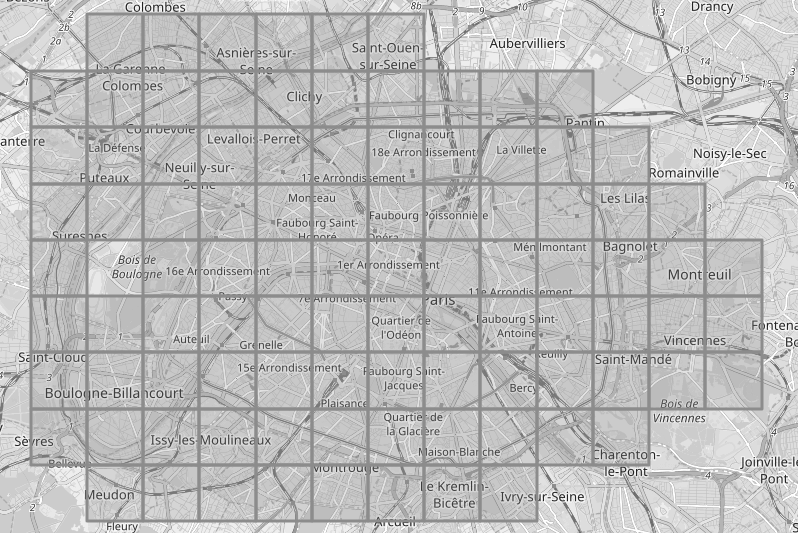
\includegraphics[width=.8\linewidth]{static/gridification_for_paris_gray.png}
\end{center}

After gridification, the ad-hoc orders within a pixel are aggregated by their
    placement timestamps into sub-daily time steps of pre-defined lengths
    to obtain a time table as exemplified in Figure \ref{f:timetable} with
    one-hour intervals.

\begin{center}
\captionof{figure}{Aggregation into a time table with hourly time steps}
\label{f:timetable}
\begin{tabular}{|c||*{9}{c|}}
    \hline
    \backslashbox{Time}{Day} & \makebox[2em]{\ldots}
        & \makebox[3em]{Mon} & \makebox[3em]{Tue}
        & \makebox[3em]{Wed} & \makebox[3em]{Thu}
        & \makebox[3em]{Fri} & \makebox[3em]{Sat}
        & \makebox[3em]{Sun} & \makebox[2em]{\ldots} \\
    \hline
    \hline
    11:00 & \ldots & $y_{11,Mon}$ & $y_{11,Tue}$ & $y_{11,Wed}$ & $y_{11,Thu}$
                   & $y_{11,Fri}$ & $y_{11,Sat}$ & $y_{11,Sun}$ & \ldots \\
    \hline
    12:00 & \ldots & $y_{12,Mon}$ & $y_{12,Tue}$ & $y_{12,Wed}$ & $y_{12,Thu}$
                   & $y_{12,Fri}$ & $y_{12,Sat}$ & $y_{12,Sun}$ & \ldots \\
    \hline
    \ldots & \ldots & \ldots & \ldots & \ldots
           & \ldots & \ldots & \ldots & \ldots & \ldots \\
    \hline
    20:00 & \ldots & $y_{20,Mon}$ & $y_{20,Tue}$ & $y_{20,Wed}$ & $y_{20,Thu}$
                   & $y_{20,Fri}$ & $y_{20,Sat}$ & $y_{20,Sun}$ & \ldots \\
    \hline
    21:00 & \ldots & $y_{21,Mon}$ & $y_{21,Tue}$ & $y_{21,Wed}$ & $y_{21,Thu}$
                   & $y_{21,Fri}$ & $y_{21,Sat}$ & $y_{21,Sun}$ & \ldots \\
    \hline
    \ldots & \ldots & \ldots & \ldots & \ldots
           & \ldots & \ldots & \ldots & \ldots & \ldots \\
    \hline
\end{tabular}
\end{center}
\

Consequently, each $y_{t,d}$ in Figure \ref{f:timetable} is the number of
    all orders within the pixel for the time of day $t$ and day of week
    $d$ ($y_t$ and $y_{t,d}$ are the same but differ in that the latter
    acknowledges a 2D view).
The same trade-off as with gridification applies:
The shorter the interval, the weaker is the demand pattern to be expected in
    the time series due to less aggregation while longer intervals lead to
    less usable forecasts.
We refer to time steps by their start time, and their number per day, $H$,
    is constant.
Given a time table as in Figure \ref{f:timetable} there are two ways to
    generate a time series by slicing:
\begin{enumerate}
    \item \textbf{Horizontal View}:
    Take only the order counts for a given time of the day
    \item \textbf{Vertical View}:
    Take all order counts and remove the double-seasonal pattern induced
    by the weekday and time of the day with decomposition
\end{enumerate}
Distinct time series are retrieved by iterating through the time tables either
    horizontally or vertically in increments of a single time step.
Another property of a generated time series is its length, which, following
    the next sub-section, can be interpreted as the sum of the production
    training set and the test day.
In summary, a distinct time series is generated from the tabular order data
    based on a configuration of parameters for the dimensions pixel size,
    number of daily time steps $H$, shape (horizontal vs. vertical), length,
    and the time step to be predicted.

\subsection{Unified Cross-Validation and Training, Validation, and Test Sets}
\label{unified_cv}

The standard $k$-fold CV, which assumes no structure in the individual
    features of the samples, as shown in $\mat{X}$ above, is adapted to the
    ordinal character of time series data:
A model must be evaluated on observations that occurred strictly after the
    ones used for training as, otherwise, the model knows about the future.
Furthermore, some models predict only a single to a few time steps before
    being retrained, while others predict an entire day without retraining
    (cf., Sub-section \ref{ml_models}).
Consequently, we must use a unified time interval wherein all forecasts are
    made first before the entire interval is evaluated.
As whole days are the longest prediction interval for models without
    retraining, we choose that as the unified time interval.
In summary, our CV methodology yields a distinct best model per pixel and day
    to be forecast.
Whole days are also practical for managers who commonly monitor, for example,
    the routing and thus the forecasting performance on a day-to-day basis.
Our methodology assumes that the models are trained at least once per day.
As we create operational forecasts into the near future in this paper,
    retraining all models with the latest available data is a logical step.

\begin{center}
\captionof{figure}{Training, validation, and test sets
                   during cross validation}
\label{f:cv}
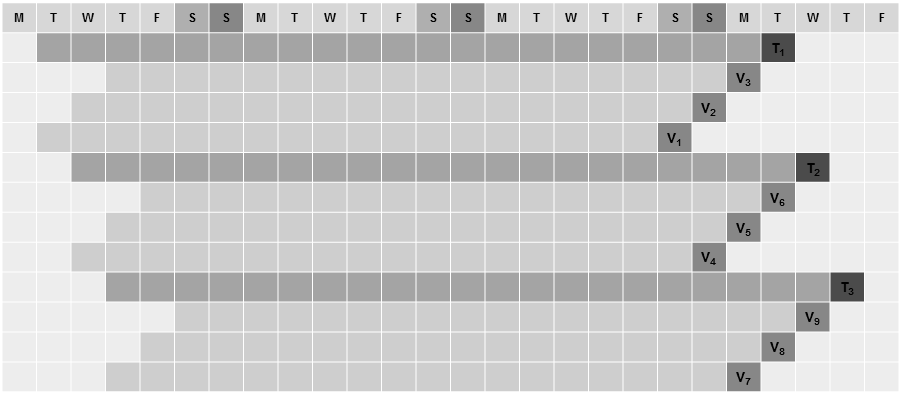
\includegraphics[width=.8\linewidth]{static/cross_validation_gray.png}
\end{center}

The training, validation, and test sets are defined as follows.
To exemplify the logic, we refer to Figure \ref{f:cv} that shows the calendar
    setup (i.e., weekdays on the x-axis) for three days $T_1$, $T_2$, and
    $T_3$ (shown in dark gray) for which we generate forecasts.
Each of these days is, by definition, a test day, and the test set comprises
    all time series, horizontal or vertical, whose last observation lies on
    that day.
With an assumed training horizon of three weeks, the 21 days before each of
    the test days constitute the corresponding training sets (shown in lighter
    gray on the same rows as $T_1$, $T_2$, and $T_3$).
There are two kinds of validation sets, depending on the decision to be made.
First, if a forecasting method needs parameter tuning, the original training
    set is divided into as many equally long series as validation days are
    needed to find stable parameters.
The example shows three validation days per test day named $V_n$ (shown
    in darker gray below each test day).
The $21 - 3 = 18$ preceding days constitute the training set corresponding to
    a validation day.
To obtain the overall validation error, the three errors are averaged.
We call these \textit{inner} validation sets because they must be repeated
    each day to re-tune the parameters and because the involved time series
    are true subsets of the original series.
Second, to find the best method per day and pixel, the same averaging logic
    is applied on the outer level.
For example, if we used two validation days to find the best method for $T_3$,
    we would average the errors of $T_1$ and $T_2$ for each method and select
    the winner; then, $T_1$ and $T_2$ constitute an \textit{outer} validation
    set.
Whereas the number of inner validation days is method-specific and must be
    chosen before generating any test day forecasts in the first place, the
    number of outer validation days may be varied after the fact and is
    determined empirically as we show in Section \ref{stu}.

Our unified CV approach is also optimized for large-scale production settings,
    for example, at companies like Uber.
As \cite{bell2018} note, there is a trade-off as to when each of the
    inner time series in the example begins.
While the forecasting accuracy likely increases with more training days,
    supporting inner series with increasing lengths, cutting the series
    to the same length allows caching the forecasts and errors.
In the example, $V_3$, $V_5$, and $V_7$, as well as $V_6$ and $V_8$ are
    identical despite belonging to different inner validation sets.
Caching is also possible on the outer level when searching for an optimal
    number of validation days for model selection.
We achieved up to 80\% cache hit ratios in our implementation in the
    empirical study, thereby saving computational resources by the same
    amount.
Lastly, we assert that our suggested CV, because of its being unified
    around whole test days and usage of fix-sized time series, is also
    suitable for creating consistent learning curves and, thus, answering
    \textbf{Q3} on the relationship between forecast accuracy and amount of
    historic data:
We simply increase the length of the outer training set holding the test day
    fixed.
Thus, independent of a method's need for parameter tuning, all methods have
    the same demand history available for each test day forecast.

\subsection{Accuracy Measures}
\label{mase}

Choosing an error measure for both model selection and evaluation is not
    straightforward when working with intermittent demand, as shown, for
    example, by \cite{syntetos2005}, and one should understand the trade-offs
    between measures.
\cite{hyndman2006} provide a study of measures with real-life data taken from
    the popular M3-competition and find that most standard measures degenerate
    under many scenarios.
They also provide a classification scheme for which we summarize the main
    points as they apply to the UDP case:
\begin{enumerate}
\item \textbf{Scale-dependent Errors}:
The error is reported in the same unit as the raw data.
Two popular examples are the root mean square error (RMSE) and mean absolute
    error (MAE).
They may be used for model selection and evaluation within a pixel, and are
    intuitively interpretable; however, they may not be used to compare errors
    of, for example, a low-demand pixel (e.g., at the UDP's service
    boundary) with that of a high-demand pixel (e.g., downtown).
\item \textbf{Percentage Errors}:
The error is derived from the percentage errors of individual forecasts per
    time step, and is also intuitively interpretable.
A popular example is the mean absolute percentage error (MAPE) that is the
    primary measure in most forecasting competitions.
Whereas such errors could be applied both within and across pixels, they
    cannot be calculated reliably for intermittent demand.
If only one time step exhibits no demand, the result is a divide-by-zero
    error.
This often occurs even in high-demand pixels due to the slicing.
\item \textbf{Relative Errors}:
A workaround is to calculate a scale-dependent error for the test day and
    divide it by the same measure calculated with forecasts of a simple
    benchmark method (e.g., na\"{i}ve method).
An example could be
    $\text{RelMAE} = \text{MAE} / \text{MAE}_\text{bm}$.
Nevertheless, even simple methods create (near-)perfect forecasts, and then
    $\text{MAE}_\text{bm}$ becomes (close to) $0$.
These numerical instabilities occurred so often in our studies that we argue
    against using such measures.
\item \textbf{Scaled Errors}:
\cite{hyndman2006} contribute this category and introduce the mean absolute
    scaled error (\gls{mase}).
It is defined as the MAE from the actual forecasting method on the test day
    (i.e., "out-of-sample") divided by the MAE from the (seasonal) na\"{i}ve
    method on the entire training set (i.e., "in-sample").
A MASE of $1$ indicates that a forecasting method has the same accuracy
    on the test day as the (seasonal) na\"{i}ve method applied on a longer
    horizon, and lower values imply higher accuracy.
Within a pixel, its results are identical to the ones obtained with MAE.
Also, we acknowledge recent publications, for example, \cite{prestwich2014} or
    \cite{kim2016}, showing other ways of tackling the difficulties mentioned.
However, only the MASE provided numerically stable results for all
    forecasts in our study.
\end{enumerate}
Consequently, we use the MASE with a seasonal na\"{i}ve benchmark as the
    primary measure in this paper.
With the previously introduced notation, it is defined as follows:
$$
\text{MASE}
:=
\frac{\text{MAE}_{\text{out-of-sample}}}{\text{MAE}_{\text{in-sample}}}
=
\frac{\text{MAE}_{\text{forecasts}}}{\text{MAE}_{\text{training}}}
=
\frac{\frac{1}{H} \sum_{h=1}^H |y_{T+h} - \hat{y}_{T+h}|}
     {\frac{1}{T-k} \sum_{t=k+1}^T |y_{t} - y_{t-k}|}
$$
The denominator can only become $0$ if the seasonal na\"{i}ve benchmark makes
    a perfect forecast on each day in the training set except the first seven
    days, which never happened in our case study involving hundreds of
    thousands of individual model trainings.
Further, as per the discussion in the subsequent Section \ref{decomp}, we also
    calculate peak-MASEs where we leave out the time steps of non-peak times
    from the calculations.
For this analysis, we define all time steps that occur at lunch (i.e., noon to
    2 pm) and dinner time (i.e., 6 pm to 8 pm) as peak.
As time steps in non-peak times typically average no or very low order counts,
    a UDP may choose to not actively forecast these at all and be rather
    interested in the accuracies of forecasting methods during peaks only.

We conjecture that percentage error measures may be usable for UDPs facing a
    higher overall demand with no intra-day down-times in between but have to
    leave that to a future study.
Yet, even with high and steady demand, divide-by-zero errors are likely to
    occur.
\subsection{Time Series Decomposition}
\label{decomp}

Concerning the time table in Figure \ref{f:timetable}, a seasonal demand
    pattern is inherent to both horizontal and vertical time series.
First, the weekday influences if people eat out or order in with our partner
    receiving more orders on Thursday through Saturday than the other four
    days.
This pattern is part of both types of time series.
Second, on any given day, demand peaks occur around lunch and dinner times.
This only regards vertical series.
Statistical analyses show that horizontally sliced time series indeed exhibit
    a periodicity of $k=7$, and vertically sliced series only yield a seasonal
    component with a regular pattern if the periodicity is set to the product
    of the number of weekdays and the daily time steps indicating a distinct
    intra-day pattern per weekday.

Figure \ref{f:stl} shows three exemplary STL decompositions for a
    $1~\text{km}^2$ pixel and a vertical time series with 60-minute time steps
    (on the x-axis) covering four weeks:
With the noisy raw data $y_t$ on the left, the seasonal and trend components,
    $s_t$ and $t_t$, are depicted in light and dark gray for increasing $ns$
    parameters.
The plots include (seasonal) na\"{i}ve forecasts for the subsequent test day
    as dotted lines.
The remainder components $r_t$ are not shown for conciseness.
The periodicity is set to $k = 7 * 12 = 84$ as our industry partner has $12$
    opening hours per day.

\begin{center}
\captionof{figure}{STL decompositions for a medium-demand pixel with hourly
                   time steps and periodicity $k=84$}
\label{f:stl}
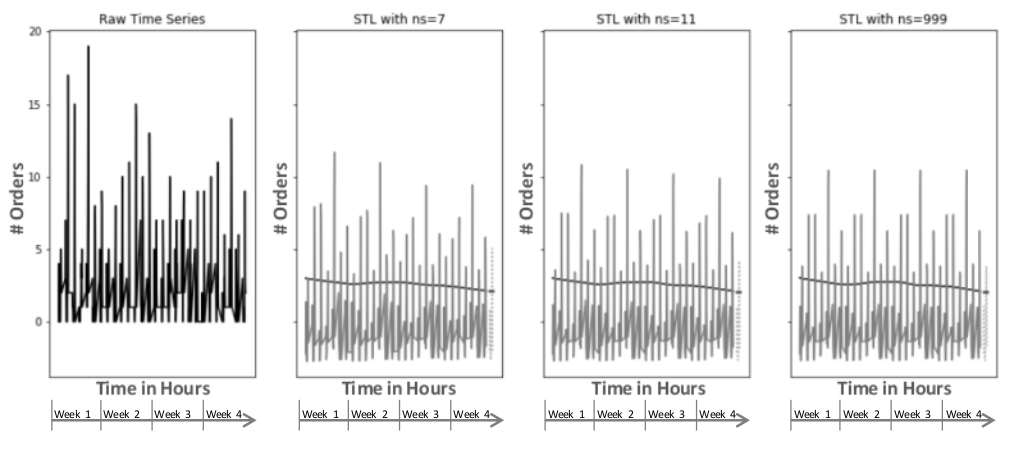
\includegraphics[width=.95\linewidth]{static/stl_gray.png}
\end{center}

As described in Sub-section \ref{stl}, with $k$ being implied by the
    application, at the very least, the length of the seasonal smoothing
    window, represented by the $ns$ parameter, must be calibrated by the
    forecaster:
It controls how many past observations go into each smoothened $s_t$.
Many practitioners, however, skip this step and set $ns$ to a big number, for
    example, $999$, then referred to as "periodic."
For the other parameters, it is common to use the default values as
    specified in \cite{cleveland1990}.
The goal is to find a decomposition with a regular pattern in $s_t$.
In Figure \ref{f:stl}, this is not true for $ns=7$ where, for
    example, the four largest bars corresponding to the same time of day a
    week apart cannot be connected by an approximately straight line.
On the contrary, a regular pattern in the most extreme way exists for
    $ns=999$, where the same four largest bars are of the same height.
This observation holds for each time step of the day.
For $ns=11$, $s_t$ exhibits a regular pattern whose bars adapt over time:
The pattern is regular as bars corresponding to the same time of day can be
    connected by approximately straight lines, and it is adaptive as these
    lines are not horizontal.
The trade-off between small and large values for $ns$ can thus be interpreted
    as allowing the average demand during peak times to change over time:
If demand is intermittent at non-peak times, it is reasonable to expect the
    bars to change over time as only the relative differences between peak and
    non-peak times impact the bars' heights with the seasonal component being
    centered around $0$.
To confirm the goodness of a decomposition statistically, one way is to verify
    that $r_t$ can be modeled as a typical error process like white noise
    $\epsilon_t$.

However, we suggest an alternative way of calibrating the STL method in an
    automated fashion based on our unified CV approach.
As hinted at in Figure \ref{f:stl}, we interpret an STL decomposition as a
    forecasting method on its own by just adding the (seasonal) na\"{i}ve
    forecasts for $s_t$ and $t_t$ and predicting $0$ for $r_t$.
Then, the $ns$ parameter is tuned just like a parameter for an ML model.
To the best of our knowledge, this has not yet been proposed before.
Conceptually, forecasting with the STL method can be viewed as a na\"{i}ve
    method with built-in smoothing, and it outperformed all other
    benchmark methods in all cases.

\subsection{Forecasting Models}
\label{models}

This sub-section describes the concrete models in our study.
Figure \ref{f:inputs} shows how we classify them into four families with
    regard to the type of the time series, horizontal or vertical, and the
    moment at which a model is trained:
Solid lines indicate that the corresponding time steps lie before the
    training, and dotted lines show the time horizon predicted by a model.
For conciseness, we only show the forecasts for one test day.
The setup is the same for each inner validation day.

\

\begin{center}
\captionof{figure}{Classification of the models by input type and training
                   moment}
\label{f:inputs}
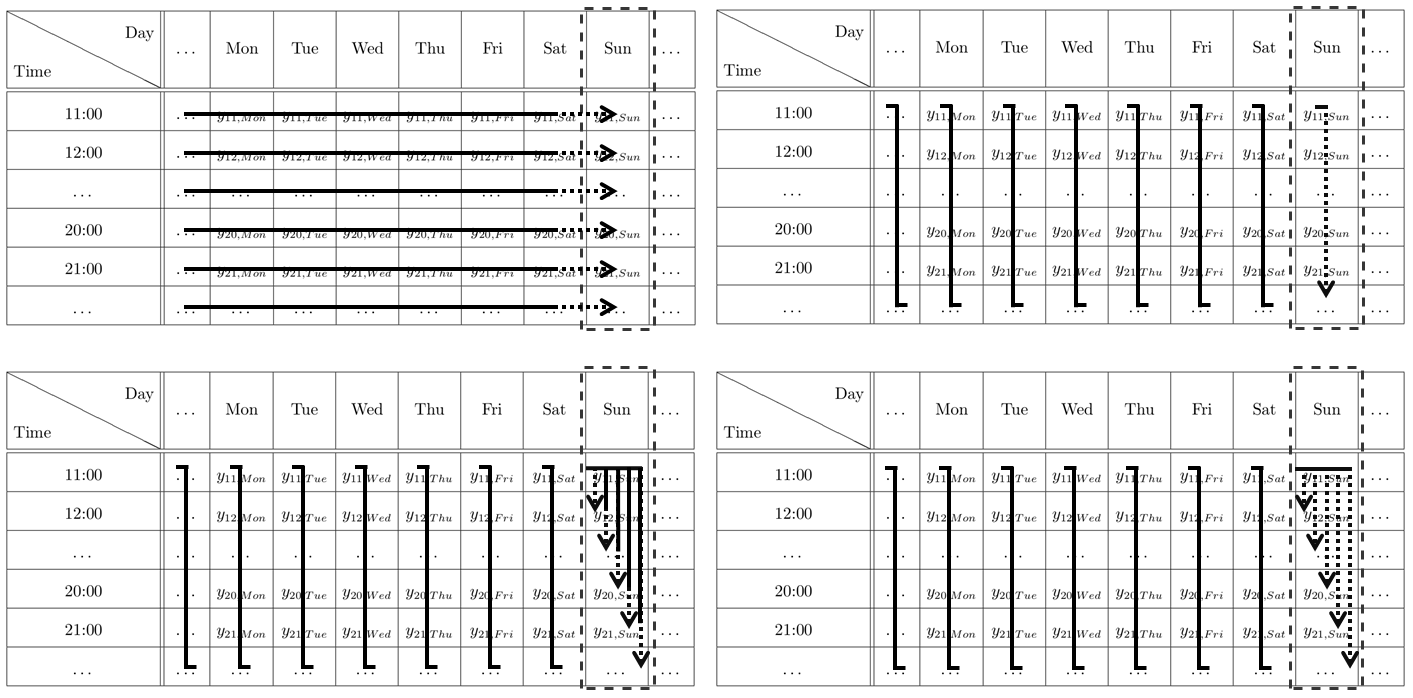
\includegraphics[width=.95\linewidth]{static/model_inputs_gray.png}
\end{center}

\subsubsection{Horizontal and Whole-day-ahead Forecasts}
\label{hori}

The upper-left in Figure \ref{f:inputs} illustrates the simplest way to
    generate forecasts for a test day before it has started:
For each time of the day, the corresponding horizontal slice becomes the input
    for a model.
With whole days being the unified time interval, each model is trained $H$
    times, providing a one-step-ahead forecast.
While it is possible to have models of a different type be selected per time
    step, that did not improve the accuracy in the empirical study.
As the models in this family do not include the test day's demand data in
    their training sets, we see them as benchmarks to answer \textbf{Q4},
    checking if a UDP can take advantage of real-time information.
The models in this family are as follows; we use prefixes, such as "h" here,
    when methods are applied in other families as well:
\begin{enumerate}
\item \textit{naive}:
          Observation from the same time step one week prior
\item \textit{trivial}:
          Predict $0$ for all time steps
\item \textit{hcroston}:
          Intermittent demand method introduced by \cite{croston1972}
\item \textit{hholt},
      \textit{hhwinters},
      \textit{hses},
      \textit{hsma}, and
      \textit{htheta}:
          Exponential smoothing without calibration
\item \textit{hets}:
          ETS calibrated as described by \cite{hyndman2008b}
\item \textit{harima}:
          ARIMA calibrated as described by \cite{hyndman2008a}
\end{enumerate}
\textit{naive} and \textit{trivial} provide an absolute benchmark for the
    actual forecasting methods.
\textit{hcroston} is often mentioned in the context of intermittent demand;
    however, the method did not perform well at all.
Besides \textit{hhwinters} that always fits a seasonal component, the
    calibration heuristics behind \textit{hets} and \textit{harima} may do so
    as well.
With $k=7$, an STL decomposition is unnecessary here.

\subsubsection{Vertical and Whole-day-ahead Forecasts without Retraining}
\label{vert}

The upper-right in Figure \ref{f:inputs} shows an alternative way to
    generate forecasts for a test day before it has started:
First, a seasonally-adjusted time series $a_t$ is obtained from a vertical
    time series by STL decomposition.
Then, the actual forecasting model, trained on $a_t$, makes an $H$-step-ahead
    prediction.
Lastly, we add the $H$ seasonal na\"{i}ve forecasts for the seasonal component
    $s_t$ to them to obtain the actual predictions for the test day.
Thus, only one training is required per model type, and no real-time data is
    used.
By decomposing the raw time series, all long-term patterns are assumed to be
    in the seasonal component $s_t$, and $a_t$ only contains the level with
    a potential trend and auto-correlations.
The models in this family are:
\begin{enumerate}
\item \textit{\gls{fnaive}},
      \textit{\gls{pnaive}}:
          Sum of STL's trend and seasonal components' na\"{i}ve forecasts
\item \textit{\gls{vholt}},
      \textit{\gls{vses}}, and
      \textit{\gls{vtheta}}:
          Exponential smoothing without calibration and seasonal
                       fit
\item \textit{\gls{vets}}:
          ETS calibrated as described by \cite{hyndman2008b}
\item \textit{\gls{varima}}:
          ARIMA calibrated as described by \cite{hyndman2008a}
\end{enumerate}
As mentioned in Sub-section \ref{unified_cv}, we include the sum of the
    (seasonal) na\"{i}ve forecasts of the STL's trend and seasonal components
    as forecasts on their own:
For \textit{fnaive}, we tune the "flexible" $ns$ parameter, and for
    \textit{pnaive}, we set it to a "periodic" value.
Thus, we implicitly assume that there is no signal in the remainder $r_t$, and
    predict $0$ for it.
\textit{fnaive} and \textit{pnaive} are two more simple benchmarks.

\subsubsection{Vertical and Real-time Forecasts with Retraining}
\label{rt}

The lower-left in Figure \ref{f:inputs} shows how models trained on vertical
    time series are extended with real-time order data as it becomes available
    during a test day:
Instead of obtaining an $H$-step-ahead forecast, we retrain a model after
    every time step and only predict one step.
The remainder is as in the previous sub-section, and the models are:
\begin{enumerate}
\item \textit{\gls{rtholt}},
      \textit{\gls{rtses}}, and
      \textit{\gls{rttheta}}:
          Exponential smoothing without calibration and seasonal fit
\item \textit{\gls{rtets}}:
          ETS calibrated as described by \cite{hyndman2008b}
\item \textit{\gls{rtarima}}:
          ARIMA calibrated as described by \cite{hyndman2008a}
\end{enumerate}
Retraining \textit{fnaive} and \textit{pnaive} did not increase accuracy, and
    thus we left them out.
A downside of this family is the significant increase in computing costs.

\subsubsection{Vertical and Real-time Forecasts without Retraining}
\label{ml_models}

The lower-right in Figure \ref{f:inputs} shows how ML models take
    real-time order data into account without retraining.
Based on the seasonally-adjusted time series $a_t$, we employ the feature
    matrix and label vector representations from Sub-section \ref{learning}
    and set $n$ to the number of daily time steps, $H$, to cover all potential
    auto-correlations.
The ML models are trained once before a test day starts.
For training, the matrix and vector are populated such that $y_T$ is set to
    the last time step of the day before the forecasts, $a_T$.
As the splitting during CV is done with whole days, the ML models are
    trained with training sets consisting of samples from all times of a day
    in an equal manner.
Thus, the ML models learn to predict each time of the day.
For prediction on a test day, the $H$ observations preceding the time
    step to be forecast are used as the input vector after seasonal
    adjustment.
As a result, real-time data are included.
The models in this family are:
\begin{enumerate}
\item \textit{vrfr}: RF trained on the matrix as described
\item \textit{vsvr}: SVR trained on the matrix as described
\end{enumerate}
We tried other ML models such as gradient boosting machines but found
    only RFs and SVRs to perform well in our study.
In the case of gradient boosting machines, this is to be expected as they are
    known not to perform well in the presence of high noise - as is natural
    with low count data - as shown, for example, by \cite{ma2018} or
    \cite{mason2000}.
Also, deep learning methods are not applicable as the feature matrices only
    consist of several hundred to thousands of rows (cf., Sub-section
    \ref{params}).
In \ref{tabular_ml_models}, we provide an alternative feature matrix
    representation that exploits the two-dimensional structure of time tables
    without decomposing the time series.
In \ref{enhanced_feats}, we show how feature matrices are extended
    to include predictors other than historical order data.
However, to answer \textbf{Q5} already here, none of the external data sources
    improves the results in our study.
Due to the high number of time series in our study, to investigate why
    no external sources improve the forecasts, we must us some automated
    approach to analyzing individual time series.
\cite{barbour2014} provide a spectral density estimation approach, called
    the Shannon entropy, that measures the signal-to-noise ratio in a
    database with a number normalized between 0 and 1 where lower values
    indicate a higher signal-to-noise ratio.
We then looked at averages of the estimates on a daily level per pixel and
    find that including any of the external data sources from
    \ref{enhanced_feats} always leads to significantly lower signal-to-noise
    ratios.
Thus, we conclude that at least for the demand faced by our industry partner
    the historical data contains all of the signal.

\section{Empirical Study: A Meal Delivery Platform in Europe}
\label{stu}

In the following, we first give a brief overview of the case study dataset
    and the parameters we applied to calibrate the time series generation.
Then, we discuss the overall results.

\subsection{Case Study Dataset}
\label{data}

The studied dataset consists of a meal delivery platform's entire
    transactional data covering the French market from launch in February of
    2016 to January of 2017.
The platform operated in five cities throughout this period and received a
    total of 686,385 orders.
The forecasting models were developed based on the data from Lyon and Paris in
    the period from August through December; this ensures comparability across
    cities and avoids irregularities in demand assumed for a new service
    within the first operating weeks.
The data exhibit a steady-state as the UDP's service area remained
    unchanged, and the numbers of orders and of couriers grew in lock-step and
    organically.
This does not mean that no new restaurants were openend: If that happened, the
    new restaurant did not attract new customers, but demand was shifted from
    other member restaurants.
Results are similar in both cities, and we only report them for Paris for
    greater conciseness.
Lastly, the platform recorded all incoming orders, and lost demand does not
    exist.
See \ref{dataset} for details on the raw data.

\subsection{Calibration of the Time Series Generation Process}
\label{params}

Independent of the concrete forecasting models, the time series generation
    must be calibrated.
We concentrate our forecasts on the pickup side for two reasons.
First, the restaurants come in a significantly lower number than the
    customers resulting in more aggregation in the order counts and thus a
    better pattern recognition.
Second, from an operational point of view, forecasts for the pickups are more
    valuable because of the waiting times due to meal preparation.
We choose pixel sizes of $0.5~\text{km}^2$, $1~\text{km}^2$, $2~\text{km}^2$,
    and $4~\text{km}^2$, and time steps covering 60, 90, and 120 minute windows
    resulting in $H_{60}=12$, $H_{90}=9$, and $H_{120}=6$ time steps per day
    with the platform operating between 11 a.m. and 11 p.m. and corresponding
    frequencies $k_{60}=7*12=84$, $k_{90}=7*9=63$, and $k_{120}=7*6=42$ for the
    vertical time series.
Smaller pixels and shorter time steps yield no recognizable patterns, yet would
    have been more beneficial for tactical routing.
90 and 120 minute time steps are most likely not desirable for routing; however,
    we keep them for comparison and note that a UDP may employ such forecasts
    to activate more couriers at short notice if a (too) high demand is
    forecasted in an hour from now.
This could, for example, be implemented by paying couriers a premium if they
    show up for work at short notice.
Discrete lengths of 3, 4, 5, 6, 7, and 8 weeks are chosen as training
    horizons.
We do so as the structure within the pixels (i.e., number and kind of
    restaurants) is not stable for more than two months in a row in the
    covered horizon.
That is confirmed by the empirical finding that forecasting accuracy
    improves with longer training horizon but this effect starts to
    level off after about six to seven weeks.
So, the demand patterns of more than two months ago do not resemble more
    recent ones.

In total, 100,000s of distinct time series are forecast in the study.

\subsection{Overall Results}
\label{overall_results}

Table \ref{t:results} summarizes the overall best-performing models grouped by
    training horizon and a pixel's average daily demand (\gls{add}) for a
    pixel size of $1~\text{km}^2$ and 60-minute time steps.
Each combination of pixel and test day counts as one case, and the total
    number of cases is denoted as $n$.
Clustering the individual results revealed that a pixel's ADD over the
    training horizon is the primary indicator of similarity and three to four
    clusters suffice to obtain cohesive clusters:
We labeled them "no", "low", "medium", and "high" demand pixels with
    increasing ADD, and present the average MASE per cluster.
The $n$ do not vary significantly across the training horizons, which confirms
    that the platform did not grow area-wise and is indeed in a steady-state.

\begin{center}
\captionof{table}{Top-3 models by training weeks and average demand
                  ($1~\text{km}^2$ pixel size, 60-minute time steps)}
\label{t:results}
\begin{tabular}{|c|c|*{12}{c|}}

\hline
\multirow{3}{*}{\rotatebox{90}{\thead{Training}}}
    & \multirow{3}{*}{\rotatebox{90}{\thead{Rank}}}
    & \multicolumn{3}{c|}{\thead{No Demand}}
    & \multicolumn{3}{c|}{\thead{Low Demand}}
    & \multicolumn{3}{c|}{\thead{Medium Demand}}
    & \multicolumn{3}{c|}{\thead{High Demand}} \\
~ & ~
    & \multicolumn{3}{c|}{(0 - 2.5)}
    & \multicolumn{3}{c|}{(2.5 - 10)}
    & \multicolumn{3}{c|}{(10 - 25)}
    & \multicolumn{3}{c|}{(25 - $\infty$)} \\
\cline{3-14}
~ & ~
    & Method & MASE & $n$
    & Method & MASE & $n$
    & Method & MASE & $n$
    & Method & MASE & $n$ \\

\hline \hline
\multirow{3}{*}{3} & 1
    & \textbf{\textit{trivial}}
        & 0.785 & \multirow{3}{*}{\rotatebox{90}{4586}}
    & \textbf{\textit{hsma}}
        & 0.819 & \multirow{3}{*}{\rotatebox{90}{2975}}
    & \textbf{\textit{hsma}}
        & 0.839 & \multirow{3}{*}{\rotatebox{90}{2743}}
    & \textbf{\textit{rtarima}}
        & 0.872 & \multirow{3}{*}{\rotatebox{90}{2018}} \\
~ & 2
    & \textit{hsma}    & 0.809 & ~
    & \textit{hses}    & 0.844 & ~
    & \textit{hses}    & 0.858 & ~
    & \textit{rtses}   & 0.873 & ~ \\
~ & 3
    & \textit{pnaive}  & 0.958 & ~
    & \textit{hets}    & 0.846 & ~
    & \textit{hets}    & 0.859 & ~
    & \textit{rtets}   & 0.877 & ~ \\

\hline
\multirow{3}{*}{4} & 1
    & \textbf{\textit{trivial}}
        & 0.770 & \multirow{3}{*}{\rotatebox{90}{4532}}
    & \textbf{\textit{hsma}}
        & 0.825 & \multirow{3}{*}{\rotatebox{90}{3033}}
    & \textbf{\textit{hsma}}
        & 0.837 & \multirow{3}{*}{\rotatebox{90}{2687}}
    & \textbf{\textit{vrfr}}
        & 0.855 & \multirow{3}{*}{\rotatebox{90}{2016}} \\
~ & 2
    & \textit{hsma}             & 0.788 & ~
    & \textit{hses}             & 0.848 & ~
    & \textit{hses}             & 0.850 & ~
    & \textbf{\textit{rtarima}} & 0.855 & ~ \\
~ & 3
    & \textit{pnaive}  & 0.917 & ~
    & \textit{hets}    & 0.851 & ~
    & \textit{hets}    & 0.854 & ~
    & \textit{rtses}   & 0.860 & ~ \\

\hline
\multirow{3}{*}{5} & 1
    & \textbf{\textit{trivial}}
        & 0.780 & \multirow{3}{*}{\rotatebox{90}{4527}}
    & \textbf{\textit{hsma}}
        & 0.841 & \multirow{3}{*}{\rotatebox{90}{3055}}
    & \textbf{\textit{hsma}}
        & 0.837 & \multirow{3}{*}{\rotatebox{90}{2662}}
    & \textbf{\textit{vrfr}}
        & 0.850 & \multirow{3}{*}{\rotatebox{90}{2019}} \\
~ & 2
    & \textit{hsma}             & 0.803 & ~
    & \textit{hses}             & 0.859 & ~
    & \textit{hets}             & 0.845 & ~
    & \textbf{\textit{rtarima}} & 0.852 & ~ \\
~ & 3
    & \textit{pnaive}  & 0.889 & ~
    & \textit{hets}    & 0.861 & ~
    & \textit{hses}    & 0.845 & ~
    & \textit{vsvr}    & 0.854 & ~ \\

\hline
\multirow{3}{*}{6} & 1
    & \textbf{\textit{trivial}}
        & 0.741 & \multirow{3}{*}{\rotatebox{90}{4470}}
    & \textbf{\textit{hsma}}
        & 0.847 & \multirow{3}{*}{\rotatebox{90}{3086}}
    & \textbf{\textit{hsma}}
        & 0.840 & \multirow{3}{*}{\rotatebox{90}{2625}}
    & \textbf{\textit{vrfr}}
        & 0.842 & \multirow{3}{*}{\rotatebox{90}{2025}} \\
~ & 2
    & \textit{hsma}             & 0.766 & ~
    & \textit{hses}             & 0.863 & ~
    & \textit{hets}             & 0.842 & ~
    & \textbf{\textit{hets}}    & 0.847 & ~ \\
~ & 3
    & \textit{pnaive}  & 0.837 & ~
    & \textit{hets}    & 0.865 & ~
    & \textit{hses}    & 0.848 & ~
    & \textit{vsvr}    & 0.848 & ~ \\

\hline
\multirow{3}{*}{7} & 1
    & \textbf{\textit{trivial}}
        & 0.730 & \multirow{3}{*}{\rotatebox{90}{4454}}
    & \textbf{\textit{hsma}}
        & 0.858 & \multirow{3}{*}{\rotatebox{90}{3132}}
    & \textbf{\textit{hets}}
        & 0.845 & \multirow{3}{*}{\rotatebox{90}{2597}}
    & \textbf{\textit{hets}}
        & 0.840 & \multirow{3}{*}{\rotatebox{90}{2007}} \\
~ & 2
    & \textit{hsma}          & 0.754 & ~
    & \textit{hses}          & 0.871 & ~
    & \textit{hsma}          & 0.847 & ~
    & \textbf{\textit{vrfr}} & 0.845 & ~ \\
~ & 3
    & \textit{pnaive}        & 0.813 & ~
    & \textit{hets}          & 0.872 & ~
    & \textbf{\textit{vsvr}} & 0.850 & ~
    & \textit{vsvr}          & 0.847 & ~ \\

\hline
\multirow{3}{*}{8} & 1
    & \textbf{\textit{trivial}}
        & 0.735 & \multirow{3}{*}{\rotatebox{90}{4402}}
    & \textbf{\textit{hsma}}
        & 0.867 & \multirow{3}{*}{\rotatebox{90}{3159}}
    & \textbf{\textit{hets}}
        & 0.846 & \multirow{3}{*}{\rotatebox{90}{2575}}
    & \textbf{\textit{hets}}
        & 0.836 & \multirow{3}{*}{\rotatebox{90}{2002}} \\
~ & 2
    & \textit{hsma}          & 0.758 & ~
    & \textit{hets}          & 0.877 & ~
    & \textbf{\textit{vsvr}} & 0.850 & ~
    & \textbf{\textit{vrfr}} & 0.842 & ~ \\
~ & 3
    & \textit{pnaive}  & 0.811 & ~
    & \textit{hses}    & 0.880 & ~
    & \textit{hsma}    & 0.851 & ~
    & \textit{vsvr}    & 0.849 & ~ \\

\hline
\end{tabular}
\end{center}
\

We use this table to answer \textbf{Q1} regarding the overall best methods
    under different ADDs.
All result tables in the main text report MASEs calculated with all time
    steps of a day.
In contrast, \ref{peak_results} shows the same tables with MASEs calculated
    with time steps within peak times only (i.e., lunch from 12 pm to 2 pm and
    dinner from 6 pm to 8 pm).
The differences lie mainly in the decimals of the individual MASE
    averages while the ranks of the forecasting methods do not change except
    in rare cases.
That shows that the presented accuracies are driven by the forecasting methods'
    accuracies at peak times.
Intuitively, they all correctly predict zero demand for non-peak times.

Unsurprisingly, the best model for pixels without demand (i.e.,
    $0 < \text{ADD} < 2.5$) is \textit{trivial}.
Whereas \textit{hsma} also adapts well, its performance is worse.
None of the more sophisticated models reaches a similar accuracy.
The intuition behind is that \textit{trivial} is the least distorted by the
    relatively large proportion of noise given the low-count nature of the
    time series.

For low demand (i.e., $2.5 < \text{ADD} < 10$), there is also a clear
    best-performing model, namely \textit{hsma}.
As the non-seasonal \textit{hses} reaches a similar accuracy as its
    potentially seasonal generalization, the \textit{hets}, we conclude that
    the seasonal pattern from weekdays is not yet strong enough to be
    recognized in low demand pixels.
So, in the absence of seasonality, models that only model a trend part are
    the least susceptible to the noise.

For medium demand (i.e., $10 < \text{ADD} < 25$) and training horizons up to
    six weeks, the best-performing models are the same as for low demand.
For longer horizons, \textit{hets} provides the highest accuracy.
Thus, to fit a seasonal pattern, longer training horizons are needed.
While \textit{vsvr} enters the top three, \textit{hets} has the edge as they
    neither require parameter tuning nor real-time data.

In summary, except for high demand, simple models trained on horizontal time
    series work best.
By contrast, high demand (i.e., $25 < \text{ADD} < \infty$) and less than
    six training weeks is the only situation where classical models trained on
    vertical time series work well.
Then, \textit{rtarima} outperforms their siblings from Sub-sections
    \ref{vert} and \ref{rt}.
We conjecture that intra-day auto-correlations as caused, for example, by
    weather, are the reason for that.
Intuitively, a certain amount of demand (i.e., a high enough signal-to-noise
    ratio) is required such that models with auto-correlations can see them
    through all the noise.
That idea is supported by \textit{vrfr} reaching a similar accuracy under
    high demand as their tree-structure allows them to fit auto-correlations.
As both \textit{rtarima} and \textit{vrfr} incorporate recent demand,
    real-time information can indeed improve accuracy.
However, once models are trained on longer horizons, \textit{hets} is more
    accurate than \textit{vrfr}.
Thus, to answer \textbf{Q4}, we conclude that real-time information only
    improves accuracy if three or four weeks of training material are
    available.

In addition to looking at the results in tables covering the entire one-year
    horizon, we also created sub-analyses on the distinct seasons spring,
    summer (incl. the long holiday season in France), and fall.
Yet, none of the results portrayed in this and the subsequent sections change
    is significant ways.
We conjecture that there could be differences if the overall demand of the UDP
    increased to a scale beyond the one this case study covers and leave that
    up to a follow-up study with a bigger UDP.

\subsection{Impact of the Training Horizon}
\label{training}

Whereas it is reasonable to assume that forecasts become more accurate as the
    training horizon expands, our study reveals some interesting findings.
First, without demand, \textit{trivial} indeed performs better with more
    training material, but improved pattern recognition cannot be the cause
    here.
Instead, we argue that the reason for this is that the longer there has been
    no steady demand, the higher the chance that this will not change soon.
Further, if we focus on shorter training horizons, the sample will necessarily
    contain cases where a pixel is initiated after a popular-to-be restaurant
    joined the platform:
Demand grows fast making \textit{trivial} less accurate, and the pixel moves
    to another cluster soon.

Second, with low demand, the best-performing \textit{hsma} becomes less
    accurate with more training material.
While one could argue that this is due to \textit{hsma} not fitting a trend,
    the less accurate \textit{hses} and \textit{hets} do fit a trend.
Instead, we argue that any low-demand time series naturally exhibits a high
    noise-to-signal ratio, and \textit{hsma} is the least susceptible to
    noise.
Then, to counter the missing trend term, the training horizon must be shorter.

With medium demand, a similar argument can be made; however, the
    signal already becomes more apparent favoring \textit{hets} with more
    training data.

Lastly, with high demand, the signal becomes so clear that more sophisticated
    models can exploit longer training horizons.

\subsection{Results by Model Families}
\label{fams}

\begin{center}
\captionof{table}{Ranking of benchmark and horizontal models
                  ($1~\text{km}^2$ pixel size, 60-minute time steps):
                  the table shows the ranks for cases with $2.5 < ADD < 25$
                  (and $25 < ADD < \infty$ in parentheses if they differ)}
\label{t:hori}
\begin{tabular}{|c|ccc|cccccccc|}
\hline
\multirow{2}{*}{\rotatebox{90}{\thead{\scriptsize{Training}}}}
    & \multicolumn{3}{c|}{\thead{Benchmarks}}
    & \multicolumn{8}{c|}{\thead{Horizontal (whole-day-ahead)}} \\
\cline{2-12}
~ & \textit{naive}     & \textit{fnaive}   & \textit{paive}
  & \textit{harima}    & \textit{hcroston} & \textit{hets} & \textit{hholt}
  & \textit{hhwinters} & \textit{hses}     & \textit{hsma} & \textit{htheta} \\
\hline \hline
3 & 11      &  7 (2) &  8 (5) & 5 (7) & 4     & 3
  &  9 (10) & 10 (9) &  2 (6) & 1     & 6 (8) \\
4 & 11      &  7 (2) &  8 (3) & 5 (6) & 4 (5) & 3 (1)
  &  9 (10) & 10 (9) &  2 (7) & 1 (4) & 6 (8) \\
5 & 11      &  7 (2) &  8 (4) & 5 (3) & 4 (9) & 3 (1)
  &  9 (10) & 10 (5) &  2 (8) & 1 (6) & 6 (7) \\
6 & 11      &  8 (5) &  9 (6) & 5 (4) & 4 (7) & 2 (1)
  & 10      &  7 (2) &  3 (8) & 1 (9) & 6 (3)  \\
7 & 11      &  8 (5) & 10 (6) & 5 (4) & 4 (7) & 2 (1)
  &  9 (10) &  7 (2) &  3 (8) & 1 (9) & 6 (3) \\
8 & 11      &  9 (5) & 10 (6) & 5 (4) & 4 (7) & 2 (1)
  &  8 (10) &  7 (2) &  3 (8) & 1 (9) & 6 (3) \\
\hline
\end{tabular}
\end{center}
\

Besides the overall results, we provide an in-depth comparison of models
    within a family.
Instead of reporting the MASE per model, we rank the models holding the
    training horizon fixed to make comparison easier.
Table \ref{t:hori} presents the models trained on horizontal time series.
In addition to \textit{naive}, we include \textit{fnaive} and \textit{pnaive}
    already here as more competitive benchmarks.
The tables in this section report two rankings simultaneously:
The first number is the rank resulting from lumping the low and medium
    clusters together, which yields almost the same rankings when analyzed
    individually.
The ranks from only high demand pixels are in parentheses if they differ.

A first insight is that \textit{fnaive} is the best benchmark in all
    scenarios:
Decomposing flexibly by tuning the $ns$ parameter is worth the computational
    cost.
Further, if one is limited in the number of non-na\"{i}ve methods,
    \textit{hets} is the best compromise and works well across all demand
    levels.
It is also the best model independent of the training horizon for high demand.
With low or medium demand, \textit{hsma} is the clear overall winner; yet,
    with high demand, models with a seasonal fit (i.e., \textit{harima},
    \textit{hets}, and \textit{hhwinters}) are more accurate, in particular,
    for longer training horizons.
This is due to demand patterns in the weekdays becoming stronger with higher
    overall demand.

\begin{center}
\captionof{table}{Ranking of classical models on vertical time series
                  ($1~\text{km}^2$ pixel size, 60-minute time steps):
                  the table shows the ranks for cases with $2.5 < ADD < 25$
                  (and $25 < ADD < \infty$ in parentheses if they differ)}
\label{t:vert}
\begin{tabular}{|c|cc|ccccc|ccccc|}
\hline
\multirow{2}{*}{\rotatebox{90}{\thead{\scriptsize{Training}}}}
    & \multicolumn{2}{c|}{\thead{Benchmarks}}
    & \multicolumn{5}{c|}{\thead{Vertical (whole-day-ahead)}}
    & \multicolumn{5}{c|}{\thead{Vertical (real-time)}} \\
\cline{2-13}
~ & \textit{hets}  & \textit{hsma}   & \textit{varima} & \textit{vets} 
  & \textit{vholt} & \textit{vses}   & \textit{vtheta} & \textit{rtarima}
  & \textit{rtets} & \textit{rtholt} & \textit{rtses}  & \textit{rttheta} \\
\hline \hline
3 &  2 (10) &  1  (7) & 6 (4) & 8 (6) & 10 (9)
  &  7  (5) & 11 (12) & 4 (1) & 5 (3) &  9 (8) & 3 (2) & 12 (11) \\
4 &  2  (8) &  1 (10) & 6 (4) & 8 (6) & 10 (9)
  &  7  (5) & 12 (11) & 3 (1) & 5 (3) &  9 (7) & 4 (2) & 11 (12) \\
5 &  2  (3) &  1 (10) & 7 (5) & 8 (7) & 10 (9)
  &  6      & 11      & 4 (1) & 5 (4) &  9 (8) & 3 (2) & 12 \\
6 &  2  (1) &  1 (10) & 6 (5) & 8 (7) & 10 (9)
  &  7  (6) & 11 (12) & 3 (2) & 5 (4) &  9 (8) & 4 (3) & 12 (11) \\
7 &  2  (1) &  1 (10) & 8 (5) & 7     & 10 (9)
  &  6      & 11 (12) &	5 (2) & 4     &  9 (8) & 3     & 12 (11) \\
8 &  2  (1) &  1  (9) & 8 (5) & 7 (6) & 10 (8)
  &  6      & 12 (10) & 5 (2) & 4     &  9 (7) & 3     & 11 \\
\hline
\end{tabular}
\end{center}
\

Table \ref{t:vert} extends the previous analysis to classical models trained
    on vertical time series.
Now, the winners from before, \textit{hets} and \textit{hsma}, serve as
    benchmarks.
Whereas for low and medium demand, no improvements can be obtained,
    \textit{rtarima} and \textit{rtses} are the most accurate with high demand
    and short training horizons.
For six or more training weeks, \textit{hets} is still optimal.
Independent of retraining and the demand level, the models' relative
    performances are consistent:
The \textit{*arima} and \textit{*ses} models are best, followed by
    \textit{*ets}, \textit{*holt}, and \textit{*theta}.
Thus, models that can deal with auto-correlations and short-term forecasting
    errors, as expressed by moving averages, and that cannot be distracted by
    trend terms are optimal for vertical series.

Finally, Table \ref{t:ml} compares the two ML-based models against the
    best-performing classical models and answers \textbf{Q2}:
With low and medium demand, no improvements can be obtained again; however,
    with high demand, \textit{vrfr} has the edge over \textit{rtarima} for
    training horizons up to six weeks.
We conjecture that \textit{vrfr} fits auto-correlations better than
    \textit{varima} and is not distracted by short-term noise as
    \textit{rtarima} may be due to the retraining.
With seven or eight training weeks, \textit{hets} remains the overall winner.
Interestingly, \textit{vsvr} is more accurate than \textit{vrfr} for low and
    medium demand.
We assume that \textit{vrfr} performs well only with strong auto-correlations,
    which are not present with low and medium demand.

\begin{center}
\captionof{table}{Ranking of ML models on vertical time series
                  ($1~\text{km}^2$ pixel size, 60-minute time steps):
                  the table shows the ranks for cases with $2.5 < ADD < 25$
                  (and $25 < ADD < \infty$ in parentheses if they differ)}
\label{t:ml}
\begin{tabular}{|c|cccc|cc|}
\hline
\multirow{2}{*}{\rotatebox{90}{\thead{\scriptsize{Training}}}}
    & \multicolumn{4}{c|}{\thead{Benchmarks}}
    & \multicolumn{2}{c|}{\thead{ML}} \\
\cline{2-7}
~ & \textit{fnaive}  & \textit{hets} & \textit{hsma}
  & \textit{rtarima} & \textit{vrfr} & \textit{vsvr} \\
\hline \hline
3 & 6     & 2 (5) & 1 (4) & 3 (1) & 5 (2) & 4 (3) \\
4 & 6 (5) & 2 (4) & 1 (6) & 3 (2) & 5 (1) & 4 (3) \\
5 & 6 (5) & 2 (4) & 1 (6) & 4 (2) & 5 (1) & 3 \\
6 & 6 (5) & 2     & 1 (6) & 4     & 5 (1) & 3 \\
7 & 6 (5) & 2 (1) & 1 (6) & 4     & 5 (2) & 3 \\
8 & 6 (5) & 2 (1) & 1 (6) & 4     & 5 (2) & 3 \\
\hline
\end{tabular}
\end{center}
\

Analogously, we created tables like Table \ref{t:hori} to \ref{t:ml} for the
    forecasts with time steps of 90 and 120 minutes and find that the relative
    rankings do not change significantly.
The same holds true for the rankings with changing pixel sizes.
For conciseness reasons, we do not include these additional tables in this
    article.
In summary, the relative performances exhibited by certain model families
    are shown to be rather stable in this case study.

\subsection{Effects of the Pixel Size and Time Step Length}
\label{pixels_intervals}

As elaborated in Sub-section \ref{grid}, more order aggregation leads to a
    higher overall demand level and an improved pattern recognition in the
    generated time series.
Consequently, individual cases tend to move to the right in tables equivalent
    to Table \ref{t:results}.
With the same $ADD$ clusters, forecasts for pixel sizes of $2~\text{km}^2$ and
    $4~\text{km}^2$ or time intervals of 90 and 120 minutes or combinations
    thereof yield results similar to the best models as revealed in Tables
    \ref{t:results}, \ref{t:hori}, \ref{t:vert}, and \ref{t:ml} for high
    demand.
By contrast, forecasts for $0.5~\text{km}^2$ pixels have most of the cases
    (i.e., $n$) in the no or low demand clusters.
In that case, the pixels are too small, and pattern recognition becomes
    harder.
While it is true, that \textit{trivial} exhibits the overall lowest MASE
    for no demand cases, these forecasts become effectively worthless for
    operations.
In the extreme, with even smaller pixels we would be forecasting $0$ orders
    in all pixels for all time steps.
In summary, the best model and its accuracy are determined primarily by the
    $ADD$, and the pixel size and interval length are merely parameters to
    control that.
The forecaster's goal is to create a grid with small enough pixels without
    losing a recognizable pattern.

\section{Conclusion}
\label{con}

We conclude this paper by elaborating on how the findings are transferable
    to similar settings, providing some implications for a UDP's
    managers, and discussing further research opportunities.

\subsection{Generalizability of the Methology and Findings}
\label{generalizability}

Whereas forecasting applications are always data-specific, the following
    aspects generalize to UDPs with ad-hoc transportation services:
\begin{itemize}
\item \textbf{Double Seasonality}:
The double seasonality causes a periodicity $k$ too large to be modeled by
    classical models, and we adapt the STL method in the \textit{fnaive} model
    such that it "flexibly" fits a seasonal pattern changing in a non-trivial
    way over time.
\item \textbf{Order Sparsity}:
The intermittent time series resulting from gridification require simple
    methods like \textit{hsma} or \textit{trivial} that are not as susceptible
    to noise as more sophisticated ones.
\item \textbf{Unified CV}:
A CV unified around a whole day allows evaluating classical statistical and ML
    methods on the same scale.
It is agnostic of both the type of the time series and retraining.
\item \textbf{Error Measure}:
Analogous to \cite{hyndman2006}, we emphasize the importance of choosing a
    consistent error measure, and argue for increased use of MASE.
\end{itemize}

\subsection{Managerial Implications}
\label{implications}

Even though zeitgeist claims that having more data is always better, our study
    shows this is not the case here:
First, under certain circumstances, accuracy may go up with shorter training
    horizons.
Second, none of the external data sources improves the accuracies.
Somewhat surprisingly, despite ML-based methods` popularity in both business
    and academia in recent years, we must conclude that classical forecasting
    methods suffice to reach the best accuracy in our study.
There is one case where ML-based methods are competitive in our case study:
    In a high demand pixel (defined as more than 25 orders per day on average),
    if only about four to six weeks of past data is available,
    the \textit{vrfr} model outperformed the classical ones.
So, we recommend trying out ML-based methods in such scenarios.
In addition, with the \textit{hsma} and \textit{hets} models being the overall
    winners, incorporating real-time data is not beneficial, in particular,
    with more than six weeks of training material available.
Lastly, with just \textit{hets}, that exhibits an accuracy comparable to
    \textit{hsma} for low and medium demand, our industry partner can likely
    schedule its shifts on an hourly basis one week in advance.

This study gives rise to the following managerial implications.
First, UDPs can implement readily available forecasting algorithms with limited
    effort.
This, however, requires purposeful data collection and preparation by those
    companies, which, according to our study, is at least equally important as
    the selection of the forecasting algorithm, as becomes clear from 
    investigating the impact of the length of the training horizon.
Second, the benefits of moving from manual forecasting to automated forecasting
    include being able to pursue a predictive routing strategy and
    demand-adjusted shift scheduling.
At the time the case study data was collected, our industry partner did not
    conduct any forecasting; the only forecasting-related activities were the
    shift managers scheduling the shifts one week in advance manually in 
    spreadsheets.
Thus, selecting the right forecasting algorithm according to the framework
    proposed in this study becomes a prerequisite to the much needed
    operational improvements UDPs need to achieve in their quest for
    profitability.
In general, many UDPs launched in recent years are venture capital backed
    start-up companies that almost by definition do not have a strong
    grounding in operational excellence, and publications such as the ones by
    Uber are the exception rather than the rule.
Our paper shows that forecasting the next couple of hours can already be
    implemented within the first year of a UDP's operations.
Even if such forecasts could not be exploited by predictive routing (e.g., due
    to prolonged waiting times at restaurants), they would help monitoring the
    operations for exceptional events.
Additionally, the shift planning may be automated saving as much as one shift
    manager per city.
We emphasize that for the most part, our proposed forecasting system
    is calibrated automatically and no manual work by a data scientist is required.
The only two parameters where assumptions need to be made are the pixel size
    and the time step.
The results in our empirical study suggest
    that a pixel size of $1~\text{km}^2$ and a time step of one hour are ideal,
    which results in the optimal trade-off
    between signal strength and spatial-temporal resolution.
Future research may explore adaptive grid-sizing depending on, for instance, demand density.
\subsection{Further Research}
\label{further_research}

Sub-sections \ref{overall_results} and \ref{fams} present the models' average
    performance.
We did not research what is the best model in a given pixel on a given day.
To answer this, a study finding an optimal number of outer validation days is
    neccessary.
With the varying effect of the training horizon, this model selection is a
    two-dimensional grid search that is prone to overfitting due to the high
    noise in low count data.
Except heuristics relating the ADD to the training horizon, we cannot say
    anything about that based on our study.
\cite{lemke2010} and \cite{wang2009} show how, for example, a time series'
    characteristics may be used to select models.
Thus, we suggest conducting more detailed analyses on how to incorporate model
    selection into our proposed forecasting system.

Future research should also integrate our forecasting system into a predictive
    routing application and evaluate its business impact.
This embeds our research into the vast literature on the VRP.
Initially introduced by \cite{dantzig1959}, VRPs are concerned with
    finding optimal routes serving customers.
We refer to \cite{toth2014} for a comprehensive overview.
The two variants relevant for the UDP case are the dynamic VRP and
    the pickup and delivery problem (PDP).
A VRP is dynamic if the data to solve a problem only becomes available
    as the operations are underway.
\cite{thomas2010}, \cite{pillac2013}, and \cite{psaraftis2016} describe how
    technological advances, in particular, mobile technologies, have led to a
    renewed interest in research on dynamic VRPs, and
    \cite{berbeglia2010} provide a general overview.
\cite{ichoua2006} and \cite{ferrucci2013} provide solution methods for
    simulation studies where they assume stochastic customer demand based on
    historical distributions.
In both studies, dummy demand nodes are inserted into the VRP instance.
Forecasts by our system extend this idea naturally as dummy nodes could be
    derived from point forecasts as well.
The concrete case of a meal delivering UDP is contained in a recent
    literature stream started by \cite{ulmer2017} and extended by
    \cite{reyes2018} and \cite{yildiz2018}: They coin the term meal delivery
    routing problem (MDRP).
The MDRP is a special case of the dynamic PDP where the defining
    characteristic is that once a vehicle is scheduled, a modification of the
    route is inadmissible.

\newpage

\appendix
\newpage
\section{Tabular and Real-time Forecasts without Retraining}
\label{tabular_ml_models}

Regarding the structure of the feature matrix for the ML models in Sub-section
    \ref{ml_models}, we provide an alternative approach that works without
    the STL method.
Instead of decomposing a time series and arranging the resulting
    seasonally-adjusted time series $a_t$ into a matrix $\mat{X}$, one can
    create a matrix with two types of feature columns mapped to the raw
    observations in $\vec{y}$:
While the first group of columns takes all observations of the same time of
    day over a horizon of, for example, one week ($n_h=7$), the second group
    takes all observations covering a pre-defined time horizon, for example
    $3$ hours ($n_r=3$ for 60-minute time steps), preceding the time step to
    be fitted.
Thus, we exploit the two-dimensional structure of time tables as well, and
    conceptually model historical and recent demand.
The alternative feature matrix appears as follows where the first three
    columns are the historical and the last three the recent demand features:

$$
\vec{y}
=
\begin{pmatrix}
    y_T \\
    y_{T-1} \\
    \dots \\
    y_{1+n_hH}
\end{pmatrix}
~~~~~
\mat{X}
=
\begin{bmatrix}
    y_{T-H}              & y_{T-2H}       & \dots & y_{T-n_hH}
        & y_{T-1}        & y_{T-2}        & \dots & y_{T-n_r} \\
    y_{T-1-H}            & y_{T-1-2H}     & \dots & y_{T-1-n_hH}
        & y_{T-2}        & y_{T-3}        & \dots & y_{T-n_r-1} \\
    \dots                & \dots          & \dots & \dots
        & \dots          & \dots          & \dots & \dots \\
    y_{1+(n_h-1)H}       & y_{1+(n_h-2)H} & \dots & y_1
        & y^*_{1+n_hH-1} & y^*_{1+n_hH-2} & \dots & y^*_{1+n_hH-n_r}
\end{bmatrix}
$$
\

Being a detail, we note that the recent demand features lying on the end of
    the previous day are set to $0$, which is shown with the $^*$ notation
    above.
This alignment of the undecomposed order data $y_t$ ensures that the ML
    models learn the two seasonal patterns independently.
The parameters $n_h$ and $n_r$ must be adapted to the data, but we found the
    above values to work well.

As such matrices resemble time tables, we refer to them as tabular.
However, we found the ML models with vertical time series to outperform the
    tabular ML models, which is why we disregarded them in the study.
This tabular form could be beneficial for UDPs with a demand that exhibits
    a weaker seasonality such as a meal delivery platform.

\newpage
\section{Enhancing Forecasting Models with External Data}
\label{enhanced_feats}

In this appendix, we show how the feature matrix in Sub-section
    \ref{ml_models} can be extended with features other than historical order
    data.
Then, we provide an overview of what external data we tried out as predictors
    in our empirical study.

\subsection{Enhanced Feature Matrices}

Feature matrices can naturally be extended by appending new feature columns
    $x_{t,f}$ or $x_f$ on the right where the former represent predictors
    changing throughout a day and the latter being static either within a
    pixel or across a city.
$f$ refers to an external predictor variable, such as one of the examples
    listed below.
In the SVR case, the columns should be standardized before fitting as external
    predictors are most likely on a different scale than the historic order
    data.
Thus, for a matrix with seasonally-adjusted order data $a_t$ in it, an
    enhanced matrix looks as follows:

$$
\vec{y}
=
\begin{pmatrix}
    a_T \\
    a_{T-1} \\
    \dots \\
    a_{H+1}
\end{pmatrix}
~~~~~
\mat{X}
=
\begin{bmatrix}
    a_{T-1}         & a_{T-2} & \dots & a_{T-H}     & ~~~
        & x_{T,A}   & \dots   & x_{B} & \dots \\
    a_{T-2}         & a_{T-3} & \dots & a_{T-(H+1)} & ~~~
        & x_{T-1,A} & \dots   & x_{B} & \dots \\
    \dots           & \dots   & \dots & \dots       & ~~~
        & \dots     & \dots   & \dots & \dots \\
    a_H             & a_{H-1} & \dots & a_1         & ~~~
        & x_{H+1,A} & \dots   & x_{B} & \dots
\end{bmatrix}
$$
\

Similarly, we can also enhance the tabular matrices from
    \ref{tabular_ml_models}.
The same comments as for their pure equivalents in Sub-section \ref{ml_models}
    apply, in particular, that ML models trained with an enhanced matrix can
    process real-time data without being retrained.
    
\subsection{External Data in the Empirical Study}
\label{external_data}

In the empirical study, we tested four groups of external features that we
    briefly describe here.

\vskip 0.1in

\textbf{Calendar Features}:
\begin{itemize}
    \item Time of day (as synthesized integers: e.g., 1,050 for 10:30 am,
                       or 1,600 for 4 pm)
    \item Day of week (as one-hot encoded booleans)
    \item Work day or not (as booleans)
\end{itemize}

\vskip 0.1in

\textbf{Features derived from the historical Order Data}:
\begin{itemize}
    \item Number of pre-orders for a time step (as integers)
    \item 7-day SMA of the percentages of discounted orders (as percentages):
          The platform is known for running marketing campaigns aimed at
          first-time customers at irregular intervals. Consequently, the
          order data show a wave-like pattern of coupons redeemed when looking
          at the relative share of discounted orders per day.
\end{itemize}

\vskip 0.1in

\textbf{Neighborhood Features}:
\begin{itemize}
    \item Ambient population (as integers) as obtained from the ORNL LandScan
          database
    \item Number of active platform restaurants (as integers)
    \item Number of overall restaurants, food outlets, retailers, and other
          businesses (as integers) as obtained from the Google Maps and Yelp
          web services
\end{itemize}

\vskip 0.1in

\textbf{Real-time Weather} (raw data obtained from IBM's
                            Wunderground database):
\begin{itemize}
    \item Absolute temperature, wind speed, and humidity
          (as decimals and percentages)
    \item Relative temperature with respect to 3-day and 7-day historical
          means (as decimals)
    \item Day vs. night defined by sunset (as booleans)
    \item Summarized description (as indicators $-1$, $0$, and $+1$)
    \item Lags of the absolute temperature and the summaries covering the
          previous three hours
\end{itemize}

\vskip 0.1in

Unfortunately, we must report that none of the mentioned external data
    improved the accuracy of the forecasts.
Some led to models overfitting the data, which could not be regulated.
Manual tests revealed that real-time weather data are the most promising
    external source.
Nevertheless, the data provided by IBM's Wunderground database originate from
    weather stations close to airports, which implies that we only have the
    same aggregate weather data for the entire city.
If weather data is available on a more granular basis in the future, we see
    some potential for exploitation.

\newpage
\section{Raw Order Data in the Case Study}
\label{dataset}

The raw data for the empirical study in Section \ref{stu} was provided by a
    meal delivery platform operating in five cities in France in 2016.
The platform received a total of 686,385 orders distributed as follows:

\
\begin{center}
\begin{tabular}{llr}
    \hline
	\thead{City} & \thead{Launch Day} & \thead{Orders} \\
	\hline
    Bordeaux & July 18 & 64,012 \\
    Lille & October 30 & 14,362 \\
    Lyon & February 21 & 214,635 \\
    Nantes & October 31 & 12,900 \\
    Paris & March 7 & 380,476 \\
\end{tabular}
\end{center}
\

The part of the database relevant for forecasting can be thought of as one
    table per city, where each row represents one order and consists of the
    following groups of columns:
\begin{enumerate}
\item \textbf{Restaurant Data}
    \begin{enumerate}
    \item unique ID and name
    \item pickup location as latitude-longitude pair
    \end{enumerate}
\item \textbf{Customer Data}
    \begin{enumerate}
    \item unique ID, name, and phone number
    \item delivery location as latitude-longitude pair (mostly physical
	      addresses but also public spots)
	\end{enumerate}
\item \textbf{Timestamps}
    \begin{enumerate}
    \item placement via the smartphone app
    \item fulfillment workflow (pickup, delivery, cancellation, re-deliveries)
    \end{enumerate}
\item \textbf{Courier Data}
    \begin{enumerate}
    \item unique ID, name, and phone number
    \item shift data (begin, breaks, end)
    \item average speed
    \end{enumerate}
\item \textbf{Order Details}
    \begin{enumerate}
    \item meals and drinks
    \item prices and discounts granted
    \end{enumerate}
\end{enumerate}

\newpage
\section{Forecasting Accuracies during Peak Times}
\label{peak_results}

This appendix shows all tables from the main text
    with the MASE averages calculated from time steps within peak times
    that are defined to be from 12 pm to 2 pm (=lunch) or from 6 pm to 8 pm (=dinner).
While the exact decimals of the MASEs differ,
    the relative ranks of the forecasting methods are the same except in rare cases.

\begin{center}
\captionof{table}{Top-3 models by training weeks and average demand
                  ($1~\text{km}^2$ pixel size, 60-minute time steps)}
\label{t:results:a}
\begin{tabular}{|c|c|*{12}{c|}}

\hline
\multirow{3}{*}{\rotatebox{90}{\thead{Training}}}
    & \multirow{3}{*}{\rotatebox{90}{\thead{Rank}}}
    & \multicolumn{3}{c|}{\thead{No Demand}}
    & \multicolumn{3}{c|}{\thead{Low Demand}}
    & \multicolumn{3}{c|}{\thead{Medium Demand}}
    & \multicolumn{3}{c|}{\thead{High Demand}} \\
~ & ~
    & \multicolumn{3}{c|}{(0 - 2.5)}
    & \multicolumn{3}{c|}{(2.5 - 10)}
    & \multicolumn{3}{c|}{(10 - 25)}
    & \multicolumn{3}{c|}{(25 - $\infty$)} \\
\cline{3-14}
~ & ~
    & Method & MASE & $n$
    & Method & MASE & $n$
    & Method & MASE & $n$
    & Method & MASE & $n$ \\

\hline \hline
\multirow{3}{*}{3} & 1
    & \textbf{\textit{trivial}}
        & 0.794 & \multirow{3}{*}{\rotatebox{90}{4586}}
    & \textbf{\textit{hsma}}
        & 0.817 & \multirow{3}{*}{\rotatebox{90}{2975}}
    & \textbf{\textit{hsma}}
        & 0.838 & \multirow{3}{*}{\rotatebox{90}{2743}}
    & \textbf{\textit{rtarima}}
        & 0.871 & \multirow{3}{*}{\rotatebox{90}{2018}} \\
~ & 2
    & \textit{hsma}    & 0.808 & ~
    & \textit{hses}    & 0.847 & ~
    & \textit{hses}    & 0.851 & ~
    & \textit{rtses}   & 0.872 & ~ \\
~ & 3
    & \textit{pnaive}  & 0.938 & ~
    & \textit{hets}    & 0.848 & ~
    & \textit{hets}    & 0.853 & ~
    & \textit{rtets}   & 0.874 & ~ \\

\hline
\multirow{3}{*}{4} & 1
    & \textbf{\textit{trivial}}
        & 0.791 & \multirow{3}{*}{\rotatebox{90}{4532}}
    & \textbf{\textit{hsma}}
        & 0.833 & \multirow{3}{*}{\rotatebox{90}{3033}}
    & \textbf{\textit{hsma}}
        & 0.839 & \multirow{3}{*}{\rotatebox{90}{2687}}
    & \textbf{\textit{vrfr}}
        & 0.848 & \multirow{3}{*}{\rotatebox{90}{2016}} \\
~ & 2
    & \textit{hsma}             & 0.794 & ~
    & \textit{hses}             & 0.838 & ~
    & \textit{hses}             & 0.847 & ~
    & \textbf{\textit{rtarima}} & 0.851 & ~ \\
~ & 3
    & \textit{pnaive}  & 0.907 & ~
    & \textit{hets}    & 0.841 & ~
    & \textit{hets}    & 0.851 & ~
    & \textit{rtses}   & 0.857 & ~ \\

\hline
\multirow{3}{*}{5} & 1
    & \textbf{\textit{trivial}}
        & 0.782 & \multirow{3}{*}{\rotatebox{90}{4527}}
    & \textbf{\textit{hsma}}
        & 0.844 & \multirow{3}{*}{\rotatebox{90}{3055}}
    & \textbf{\textit{hsma}}
        & 0.841 & \multirow{3}{*}{\rotatebox{90}{2662}}
    & \textbf{\textit{vrfr}}
        & 0.849 & \multirow{3}{*}{\rotatebox{90}{2019}} \\
~ & 2
    & \textit{hsma}             & 0.802 & ~
    & \textit{hses}             & 0.851 & ~
    & \textit{hets}             & 0.844 & ~
    & \textbf{\textit{rtarima}} & 0.851 & ~ \\
~ & 3
    & \textit{pnaive}  & 0.888 & ~
    & \textit{hets}    & 0.863 & ~
    & \textit{hses}    & 0.845 & ~
    & \textit{vsvr}    & 0.853 & ~ \\

\hline
\multirow{3}{*}{6} & 1
    & \textbf{\textit{trivial}}
        & 0.743 & \multirow{3}{*}{\rotatebox{90}{4470}}
    & \textbf{\textit{hsma}}
        & 0.843 & \multirow{3}{*}{\rotatebox{90}{3086}}
    & \textbf{\textit{hsma}}
        & 0.841 & \multirow{3}{*}{\rotatebox{90}{2625}}
    & \textbf{\textit{vrfr}}
        & 0.844 & \multirow{3}{*}{\rotatebox{90}{2025}} \\
~ & 2
    & \textit{hsma}             & 0.765 & ~
    & \textit{hses}             & 0.853 & ~
    & \textit{hses}             & 0.844 & ~
    & \textbf{\textit{hets}}    & 0.847 & ~ \\
~ & 3
    & \textit{pnaive}  & 0.836 & ~
    & \textit{hets}    & 0.861 & ~
    & \textit{hets}    & 0.844 & ~
    & \textit{vsvr}    & 0.849 & ~ \\

\hline
\multirow{3}{*}{7} & 1
    & \textbf{\textit{trivial}}
        & 0.728 & \multirow{3}{*}{\rotatebox{90}{4454}}
    & \textbf{\textit{hsma}}
        & 0.855 & \multirow{3}{*}{\rotatebox{90}{3132}}
    & \textbf{\textit{hets}}
        & 0.843 & \multirow{3}{*}{\rotatebox{90}{2597}}
    & \textbf{\textit{hets}}
        & 0.839 & \multirow{3}{*}{\rotatebox{90}{2007}} \\
~ & 2
    & \textit{hsma}          & 0.744 & ~
    & \textit{hses}          & 0.862 & ~
    & \textit{hsma}          & 0.845 & ~
    & \textbf{\textit{vrfr}} & 0.842 & ~ \\
~ & 3
    & \textit{pnaive}        & 0.812 & ~
    & \textit{hets}          & 0.868 & ~
    & \textbf{\textit{vsvr}} & 0.849 & ~
    & \textit{vsvr}          & 0.846 & ~ \\

\hline
\multirow{3}{*}{8} & 1
    & \textbf{\textit{trivial}}
        & 0.736 & \multirow{3}{*}{\rotatebox{90}{4402}}
    & \textbf{\textit{hsma}}
        & 0.865 & \multirow{3}{*}{\rotatebox{90}{3159}}
    & \textbf{\textit{hets}}
        & 0.843 & \multirow{3}{*}{\rotatebox{90}{2575}}
    & \textbf{\textit{hets}}
        & 0.837 & \multirow{3}{*}{\rotatebox{90}{2002}} \\
~ & 2
    & \textit{hsma}          & 0.759 & ~
    & \textit{hets}          & 0.874 & ~
    & \textbf{\textit{vsvr}} & 0.848 & ~
    & \textbf{\textit{vrfr}} & 0.841 & ~ \\
~ & 3
    & \textit{pnaive}  & 0.820 & ~
    & \textit{hses}    & 0.879 & ~
    & \textit{hsma}    & 0.850 & ~
    & \textit{vsvr}    & 0.847 & ~ \\

\hline
\end{tabular}
\end{center}

\begin{center}
\captionof{table}{Ranking of benchmark and horizontal models
                  ($1~\text{km}^2$ pixel size, 60-minute time steps):
                  the table shows the ranks for cases with $2.5 < ADD < 25$
                  (and $25 < ADD < \infty$ in parentheses if they differ)}
\label{t:hori:a}
\begin{tabular}{|c|ccc|cccccccc|}
\hline
\multirow{2}{*}{\rotatebox{90}{\thead{\scriptsize{Training}}}}
    & \multicolumn{3}{c|}{\thead{Benchmarks}}
    & \multicolumn{8}{c|}{\thead{Horizontal (whole-day-ahead)}} \\
\cline{2-12}
~ & \textit{naive}     & \textit{fnaive}   & \textit{paive}
  & \textit{harima}    & \textit{hcroston} & \textit{hets} & \textit{hholt}
  & \textit{hhwinters} & \textit{hses}     & \textit{hsma} & \textit{htheta} \\
\hline \hline
3 & 11      &  7 (2) &  8 (5) & 5 (7) & 4     & 3
  &  9 (10) & 10 (9) &  2 (6) & 1     & 6 (8) \\
4 & 11      &  7 (2) &  8 (3) & 5 (6) & 4 (5) & 3 (1)
  &  9 (10) & 10 (9) &  2 (8) & 1 (4) & 6 (7) \\
5 & 11      &  7 (2) &  8 (4) & 5 (3) & 4 (9) & 3 (1)
  &  9 (10) & 10 (5) &  2 (8) & 1 (6) & 6 (7) \\
6 & 11      &  8 (5) &  9 (6) & 5 (4) & 4 (7) & 2 (1)
  & 10      &  7 (2) &  3 (8) & 1 (9) & 6 (3)  \\
7 & 11      &  8 (5) & 10 (6) & 5 (4) & 4 (7) & 2 (1)
  &  9 (10) &  7 (2) &  3 (8) & 1 (9) & 6 (3) \\
8 & 11      &  9 (5) & 10 (6) & 5 (4) & 4 (7) & 2 (1)
  &  8 (10) &  7 (2) &  3 (8) & 1 (9) & 6 (3) \\
\hline
\end{tabular}
\end{center}
\

\begin{center}
\captionof{table}{Ranking of classical models on vertical time series
                  ($1~\text{km}^2$ pixel size, 60-minute time steps):
                  the table shows the ranks for cases with $2.5 < ADD < 25$
                  (and $25 < ADD < \infty$ in parentheses if they differ)}
\label{t:vert:a}
\begin{tabular}{|c|cc|ccccc|ccccc|}
\hline
\multirow{2}{*}{\rotatebox{90}{\thead{\scriptsize{Training}}}}
    & \multicolumn{2}{c|}{\thead{Benchmarks}}
    & \multicolumn{5}{c|}{\thead{Vertical (whole-day-ahead)}}
    & \multicolumn{5}{c|}{\thead{Vertical (real-time)}} \\
\cline{2-13}
~ & \textit{hets}  & \textit{hsma}   & \textit{varima} & \textit{vets} 
  & \textit{vholt} & \textit{vses}   & \textit{vtheta} & \textit{rtarima}
  & \textit{rtets} & \textit{rtholt} & \textit{rtses}  & \textit{rttheta} \\
\hline \hline
3 &  2 (10) &  1  (7) & 6 (4) & 8 (6) & 10 (9)
  &  7  (5) & 11 (12) & 4 (1) & 5 (3) &  9 (8) & 3 (2) & 12 (11) \\
4 &  2  (7) &  1 (10) & 6 (4) & 8 (6) & 10 (9)
  &  7  (5) & 12 (11) & 3 (1) & 5 (3) &  9 (8) & 4 (2) & 11 (12) \\
5 &  2  (3) &  1 (10) & 7 (5) & 8 (7) & 10 (9)
  &  6      & 11      & 4 (1) & 5 (4) &  9 (8) & 3 (2) & 12 \\
6 &  2  (1) &  1 (10) & 6 (5) & 8 (7) & 10 (9)
  &  7  (6) & 11 (12) & 3 (2) & 5 (4) &  9 (8) & 4 (3) & 12 (11) \\
7 &  2  (1) &  1 (10) & 8 (5) & 7     & 10 (9)
  &  6      & 11 (12) &	5 (2) & 4     &  9 (8) & 3     & 12 (11) \\
8 &  2  (1) &  1  (9) & 8 (5) & 7     & 10 (8)
  &  6      & 12 (10) & 5 (2) & 4     &  9 (6) & 3     & 11 \\
\hline
\end{tabular}
\end{center}
\

\pagebreak

\begin{center}
\captionof{table}{Ranking of ML models on vertical time series
                  ($1~\text{km}^2$ pixel size, 60-minute time steps):
                  the table shows the ranks for cases with $2.5 < ADD < 25$
                  (and $25 < ADD < \infty$ in parentheses if they differ)}
\label{t:ml:a}
\begin{tabular}{|c|cccc|cc|}
\hline
\multirow{2}{*}{\rotatebox{90}{\thead{\scriptsize{Training}}}}
    & \multicolumn{4}{c|}{\thead{Benchmarks}}
    & \multicolumn{2}{c|}{\thead{ML}} \\
\cline{2-7}
~ & \textit{fnaive}  & \textit{hets} & \textit{hsma}
  & \textit{rtarima} & \textit{vrfr} & \textit{vsvr} \\
\hline \hline
3 & 6     & 2 (5) & 1 (3) & 3 (1) & 5 (2) & 4 \\
4 & 6 (5) & 2 (3) & 1 (6) & 3 (2) & 5 (1) & 4 \\
5 & 6 (5) & 2 (4) & 1 (6) & 4 (2) & 5 (1) & 3 \\
6 & 6 (5) & 2     & 1 (6) & 4     & 5 (1) & 3 \\
7 & 6 (5) & 2 (1) & 1 (6) & 4     & 5 (2) & 3 \\
8 & 6 (5) & 2 (1) & 1 (6) & 4     & 5 (2) & 3 \\
\hline
\end{tabular}
\end{center}
\

\newpage
\section{Glossary}
\label{glossary}

% Abbreviations for technical terms.
\newglossaryentry{add}{
    name=ADD, description={Average Daily Demand}
}
\newglossaryentry{cart}{
    name=CART, description={Classification and Regression Trees}
}
\newglossaryentry{cv}{
    name=CV, description={Cross Validation}
}
\newglossaryentry{mase}{
    name=MASE, description={Mean Absolute Scaled Error}
}
\newglossaryentry{mdrp}{
    name=MDRP, description={Meal Delivery Routing Proplem}
}
\newglossaryentry{ml}{
    name=ML, description={Machine Learning}
}
\newglossaryentry{pdp}{
    name=PDP, description={Pickup and Delivery Problem}
}
\newglossaryentry{rf}{
    name=RF,  description={Random Forest}
}
\newglossaryentry{stl}{
    name=STL, description={Seasonal and Trend Decomposition using Loess}
}
\newglossaryentry{svm}{
    name=SVM, description={Support Vector Machine}
}
\newglossaryentry{svr}{
    name=SVR, description={Support Vector Regression}
}
\newglossaryentry{udp}{
    name=UDP, description={Urban Delivery Platform}
}
\newglossaryentry{vrp}{
    name=VRP, description={Vehicle Routing Problem}
}

% Model names.
\newglossaryentry{naive}{
    name=naive, description={(Seasonal) Na\"{i}ve Method}
}
\newglossaryentry{fnaive}{
    name=fnaive, description={"Flexible" STL Decomposition,
                              with tuned ns parameter}
}
\newglossaryentry{pnaive}{
    name=pnaive, description={"Periodic" STL Decomposition,
                              with ns parameter set to large number}
}
\newglossaryentry{trivial}{
    name=trivial, description={Trivial Method}
}
\newglossaryentry{hcroston}{
    name=hcroston, description={Croston's Method,
                                trained on horizontal time series}
}
\newglossaryentry{hholt}{
    name=hholt, description={Holt's Linear Trend Method,
                             trained on horizontal time series}
}
\newglossaryentry{vholt}{
    name=vholt, description={Holt's Linear Trend Method,
                             trained on vertical time series}
}
\newglossaryentry{rtholt}{
    name=rtholt, description={Holt's Linear Trend Method,
                              (re)trained on vertical time series}
}
\newglossaryentry{hhwinters}{
    name=hhwinters, description={Holt-Winter's Seasonal Method,
                                 trained on horizontal time series}
}
\newglossaryentry{hses}{
    name=hses, description={Simple Exponential Smoothing Method,
                            trained on horizontal time series}
}
\newglossaryentry{vses}{
    name=vses, description={Simple Exponential Smoothing Method,
                            trained on vertical time series}
}
\newglossaryentry{rtses}{
    name=rtses, description={Simple Exponential Smoothing Method,
                             (re)trained on vertical time series}
}
\newglossaryentry{hsma}{
    name=hsma, description={Simple Moving Average Method,
                            trained on horizontal time series}
}
\newglossaryentry{htheta}{
    name=htheta, description={Theta Method,
                              trained on horizontal time series}
}
\newglossaryentry{vtheta}{
    name=vtheta, description={Theta Method,
                              trained on vertical time series}
}
\newglossaryentry{rttheta}{
    name=rttheta, description={Theta Method,
                               (re)trained on vertical time series}
}
\newglossaryentry{hets}{
    name=hets, description={ETS State Space Method,
                            trained on horizontal time series}
}
\newglossaryentry{vets}{
    name=vets, description={ETS State Space Method,
                            trained on vertical time series}
}
\newglossaryentry{rtets}{
    name=rtets, description={ETS State Space Method,
                             (re)trained on vertical time series}
}
\newglossaryentry{harima}{
    name=harima, description={Autoregressive Integrated Moving Average
                              Method,
                              trained on horizontal time series}
}
\newglossaryentry{varima}{
    name=varima, description={Autoregressive Integrated Moving Average
                              Method,
                              trained on vertical time series}
}
\newglossaryentry{rtarima}{
    name=rtarima, description={Autoregressive Integrated Moving Average
                               Method,
                               (re)trained on vertical time series}
}
\newglossaryentry{vrfr}{
    name=vrfr, description={Random Forest Regression Method,
                            trained on vertical time series}
}
\newglossaryentry{vsvr}{
    name=vsvr, description={Support Vector Regression Method,
                            trained on vertical time series}
}

\printglossary[title=]
\newpage

\bibliographystyle{static/elsarticle-harv}
\bibliography{tex/references}

\end{document}